The observed data along with the prediction for a SM Higgs boson with m(H)=125.0 $\GeV$ and the expected background in each differential bin for
the chosen observables are shown in Figures ~\ref{fig:differential-bins} and~\ref{fig:differential-bins-2} for production and decay related observables
respectively. The differential results are only produced using 8~TeV data due to limited statistics of 7~TeV data. 
The extracted measurements of differential fiducial cross section for production and decay related observables are shown in Figures
~\ref{fig:differential-results} and~\ref{fig:differential-results-2} respectively. For production related observables, the results are produced for 
four-leptons transverse momentum and rapidity, transverse momentum of leading jet, jet multiplicity and separation between the leading jet and the 
Higgs candidate. 
The uncertainty in the theoretical prediction for the dominant $\ggH$ process is estimated in each bin of the studied observable with the generator
used for the specific signal description ({\sc HRes}, {\sc powheg minlo-HJ}, or  {\sc powheg+JHUgen}). 
The uncertainty in the theoretical prediction for the associated production mechanisms are assumed to be constant among differential bins and 
are obtained from Ref.~\cite{LHCHiggsCrossSectionWorkingGroup:2013tqa}.
The differential cross sections as a function of four-leptons transverse momentum and rapidity are sensitive to perturbative QCD calculations of
the the dominant loop-mediated $\ggH$ production mode, in which Higgs transverse momentum $p_T(H)$ is anticipated to be balanced with the emission 
of soft quarks and gluons. The differential distribution as a function rapidity of four-lepton system also probes  the PDFs of the colliding protons
and representation of the gluon fusion production modes. The differential observables, transverse momentum of leading jet, jet multiplicity N(jets) and 
difference of rapidity between leading jet and Higgs candidate probes to hard quark and gluon radiation theoretical modelling in this process, 
comparative contribution of different Higgs production modes. The comparison of the measurements with theoretical predictions
from {\sc hres}, {\sc powheg+JHUgen} and {\sc minloHJ} for the gg$\rightarrow$H process (shown in pink, blue and yellow, respectively) together with
the predictions for XH $=$ VBF ({\sc powheg}) $+$ VH $+$ ttH({\sc pythia}) (shown in green) is also shown. The error bars represents  
statistical and systematic uncertainty, while the grey box represents the additional uncertainty incurred when using different models to unfold 
the observed data distribution back to particle level. The results are found to be compatible with SM based theoretical predictions within big 
uncertainties.  Although the observables considered for the differential measurement are sensitive to the higher order QCD effects and to the proton PDF, 
the present data does not allow one to discriminate between generators used to describe the dominant $\ggH$ process.
\par 
When extracting the differential fiducial cross sections, the fractions
of the $4e,4\mu$ and $2e2\mu$ contributions to the fiducial cross sections in each bin is allowed to float. 
Results where the fractions are fixed to their SM expectations are included in Appendix~\ref{app:fixfrac}. Similarly, results
where the model dependence uncertainty is assessed by taking into account the experimental constraints from the exiting CMS measurements are included in
Appendix~\ref{fig:differential-results-restrictive_md}. 
The largest deviation from the SM based predictions is observed in case of the jet multiplicity differential cross section, with p-value that quantifies
the compatibility between data and predictions $p=0.13$. The p-value was computed from the difference between the $-2\log(\mathcal{L})$ at its best-fit
value and the value with the cross sections fixed to the theory prediction. 
\begin{figure}[!htb]
  \begin{center}
    \subfigure[$\pt(\mathrm{H})$]{
      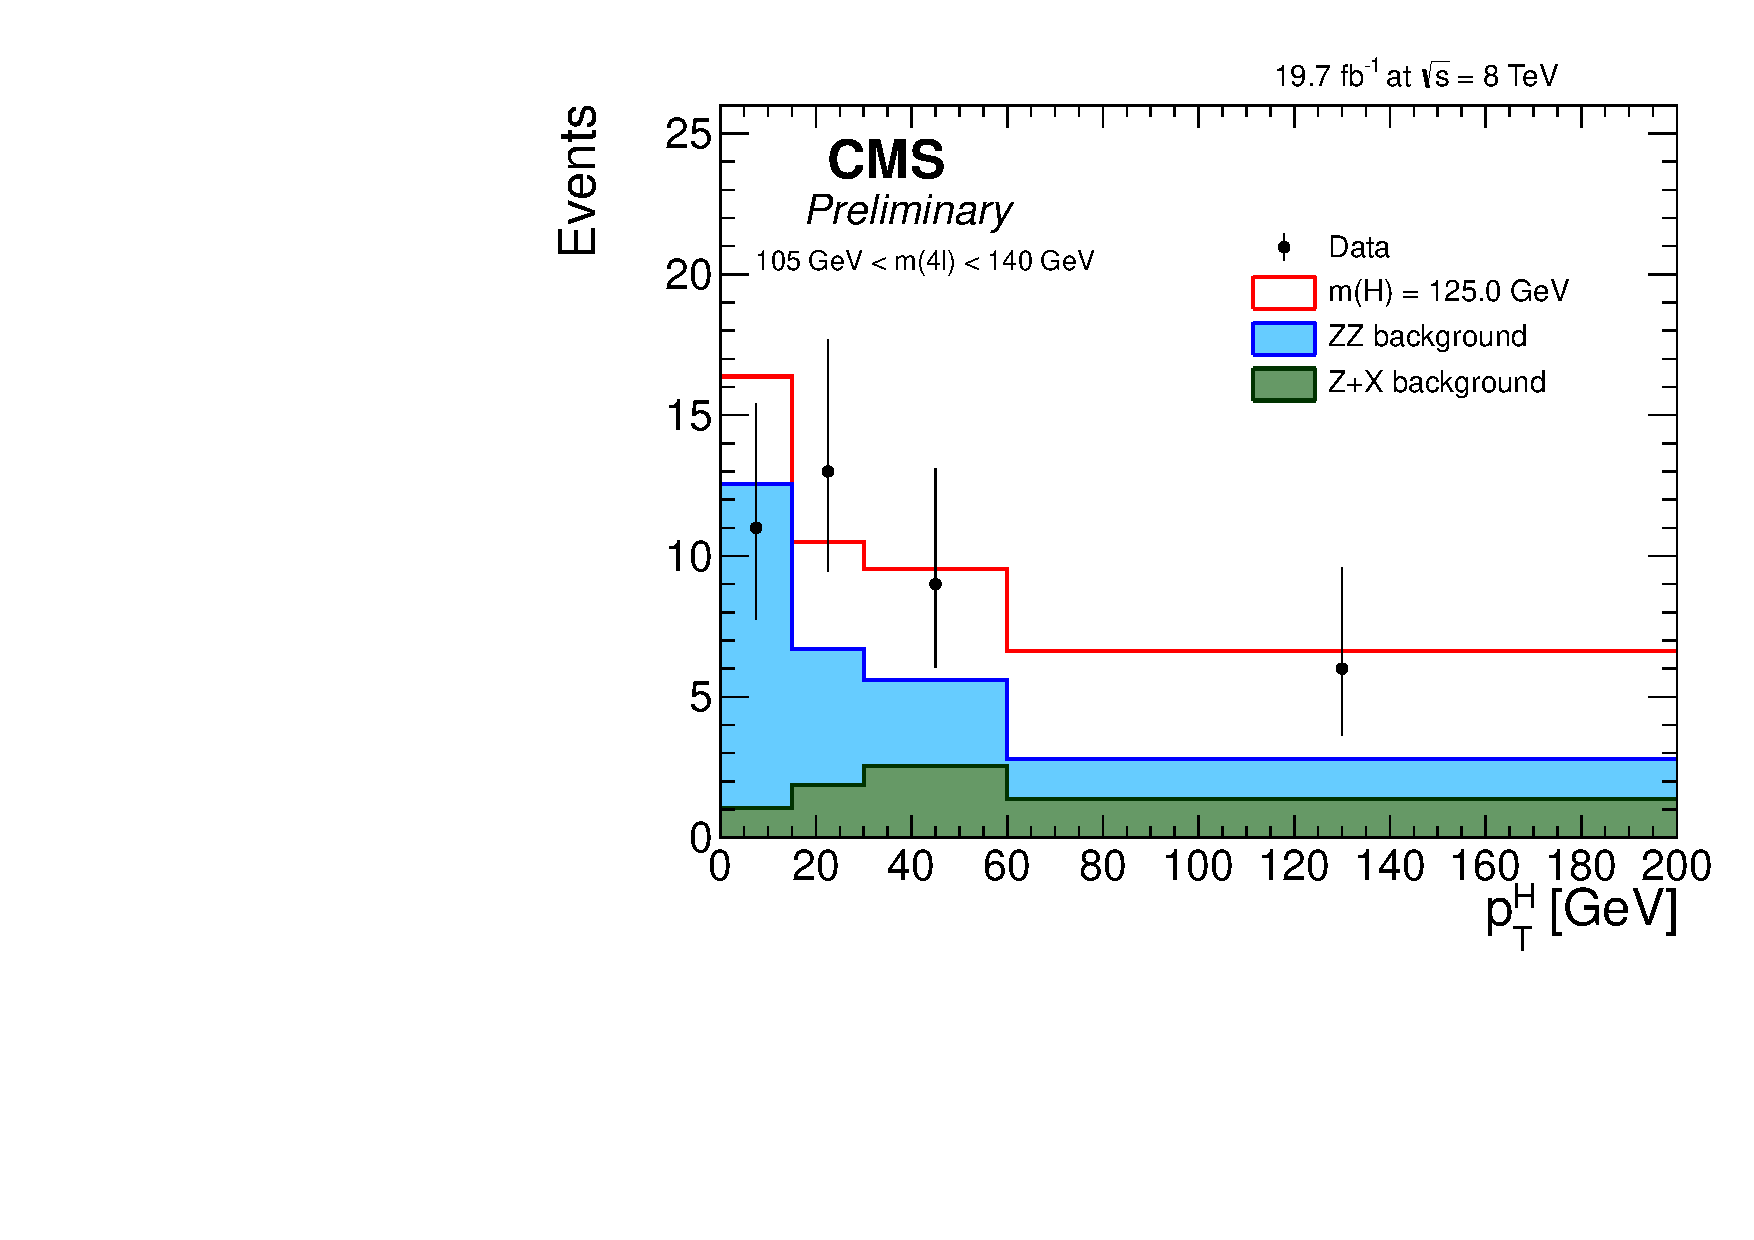
\includegraphics[width=0.33\textwidth,angle=0]{Plots/data_pT4l_4l.pdf}
      \label{fig:differential-bins:a}
    }
    \subfigure[$|y(\mathrm{H})|$]{
      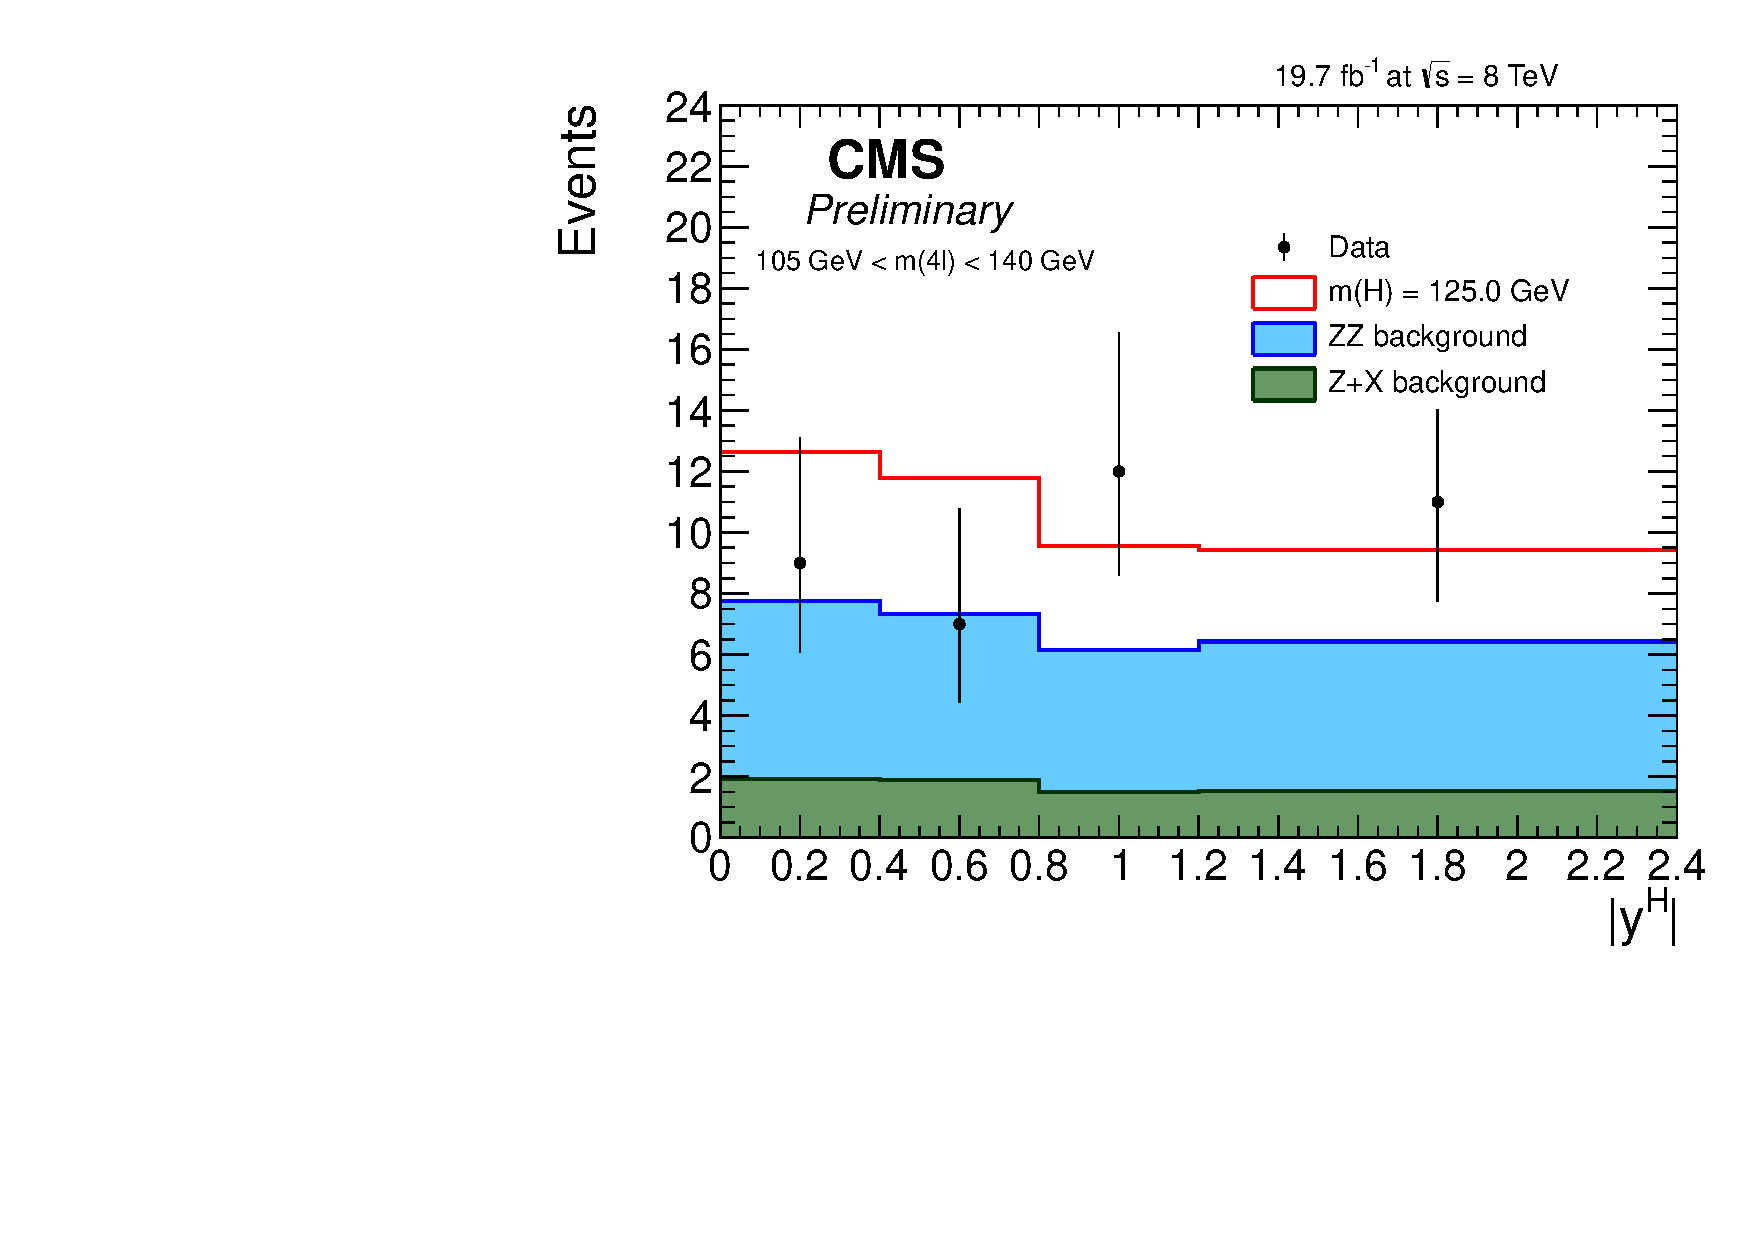
\includegraphics[width=0.33\textwidth,angle=0]{Plots/data_rapidity4l_4l.pdf}
      \label{fig:differential-bins:b}
    } 
    \subfigure[N(jets), $|\eta|<4.7$]{
      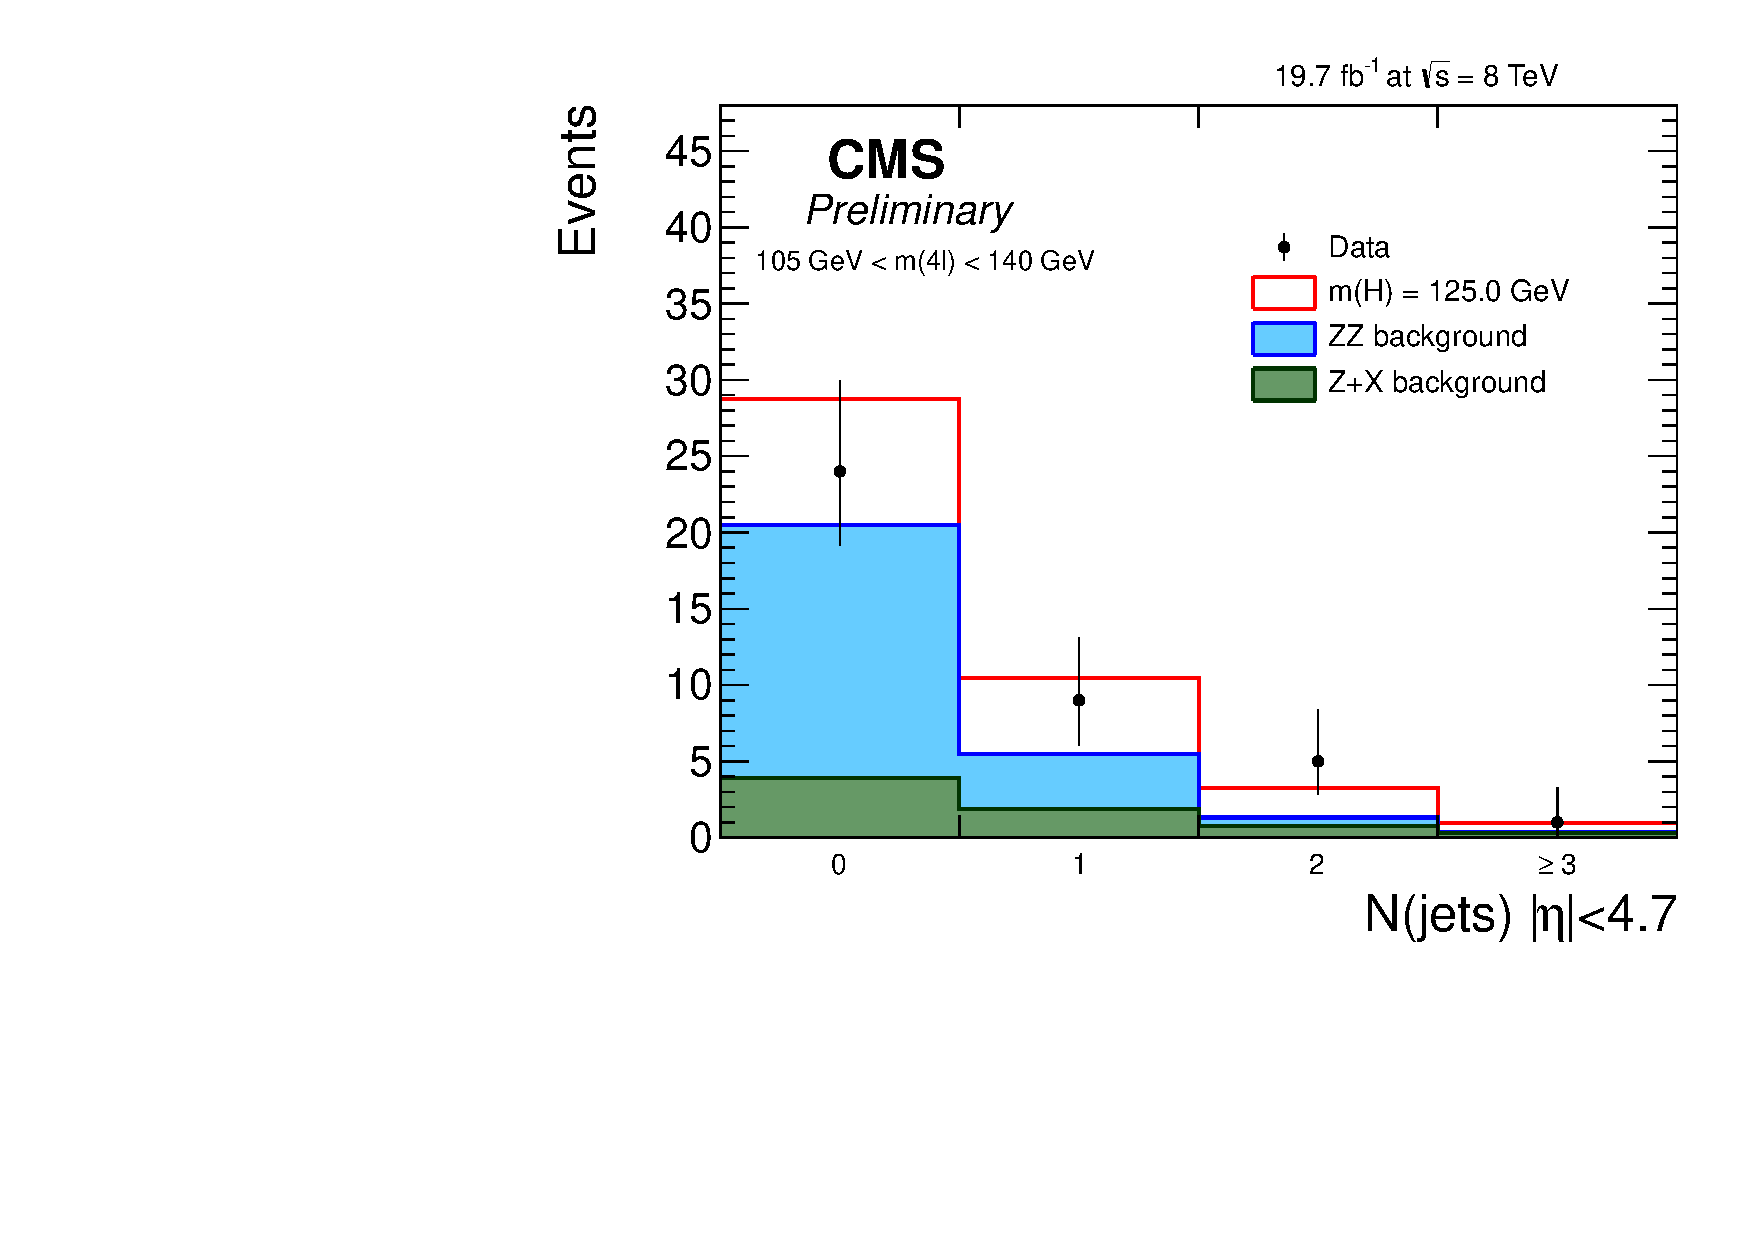
\includegraphics[width=0.33\textwidth,angle=0]{Plots/data_njets_reco_pt30_eta4p7_4l.pdf}
      \label{fig:differential-bins:e}                                                                                                                            
    } \\
    \subfigure[$\pt(\mathrm{jet})$]{
      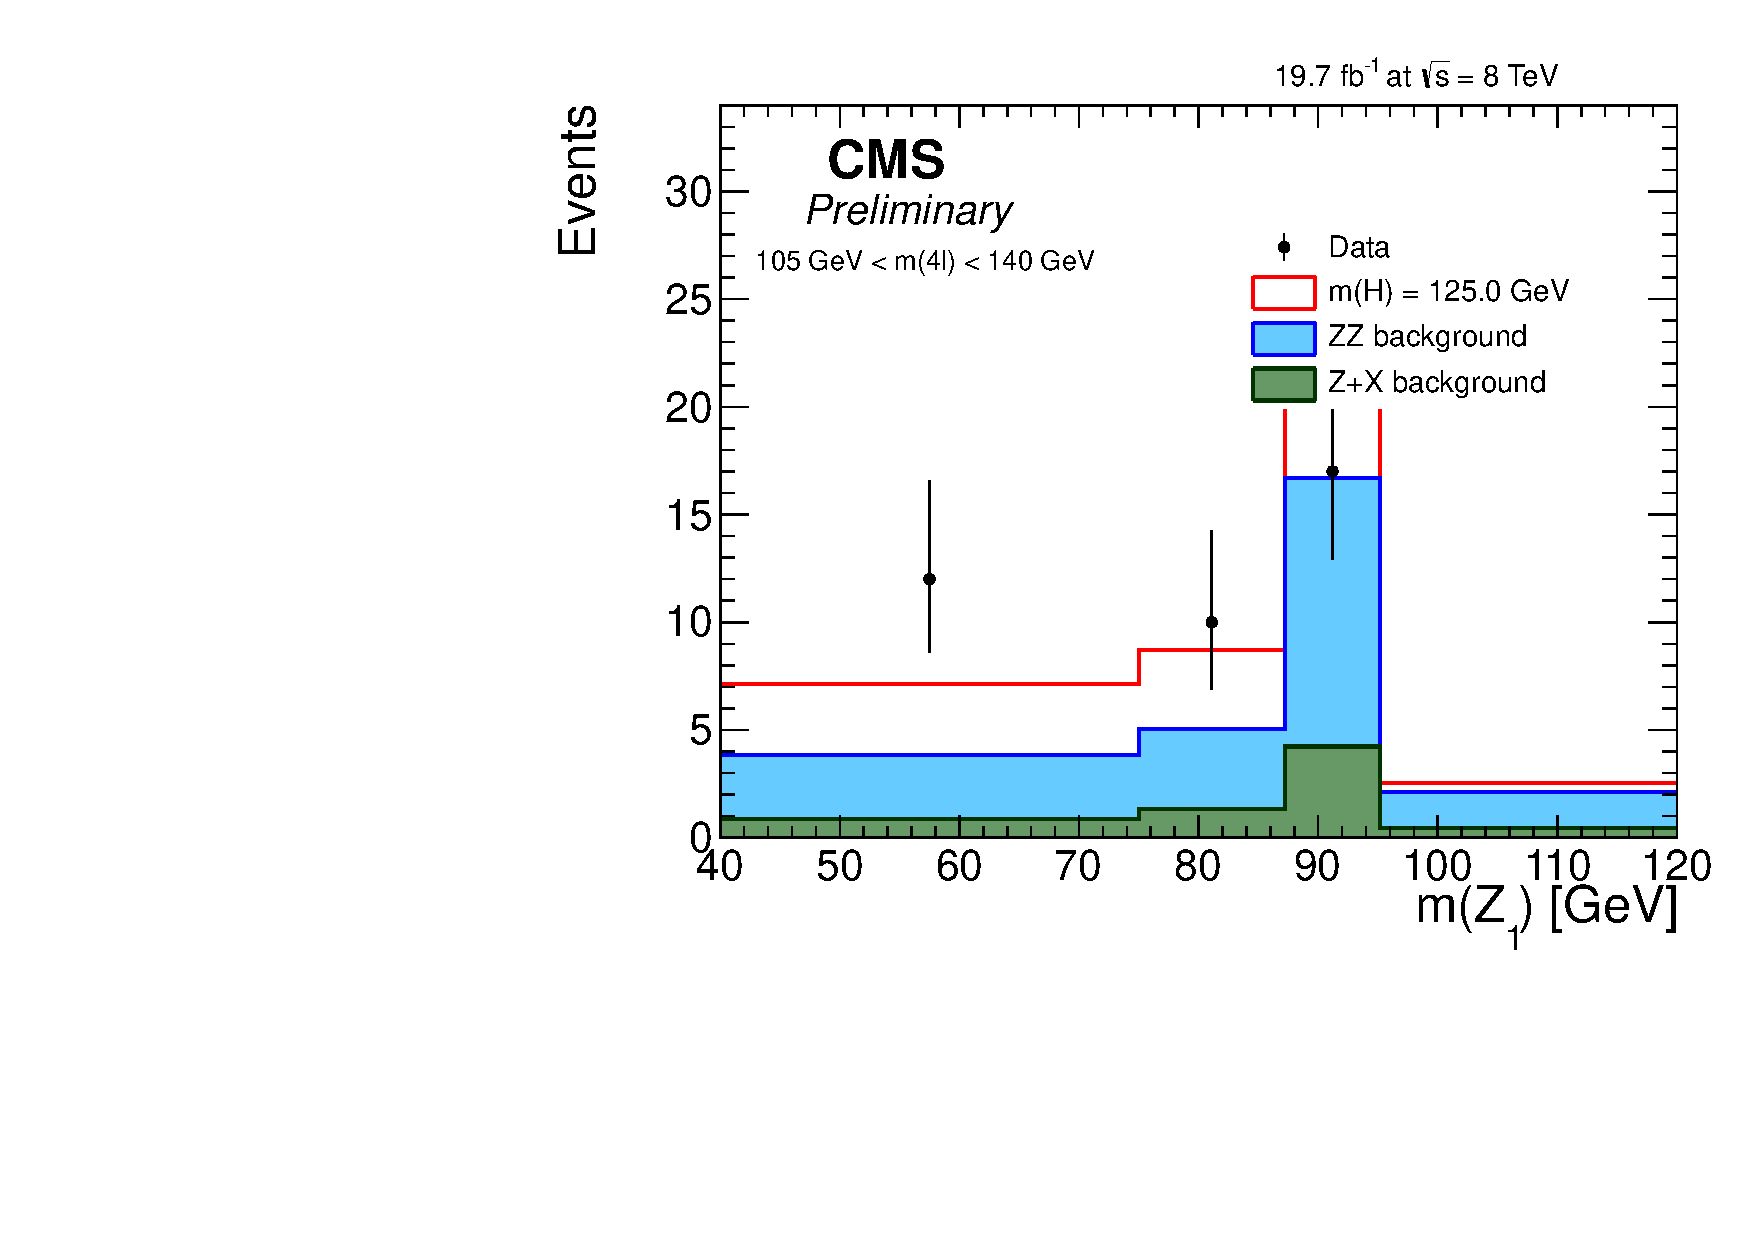
\includegraphics[width=0.33\textwidth,angle=0]{Plots/data_massZ1_4l.pdf}
      \label{fig:differential-bins:c}
    }
    \subfigure[$|y(\mathrm{H}) - y(\mathrm{jet})|$]{
      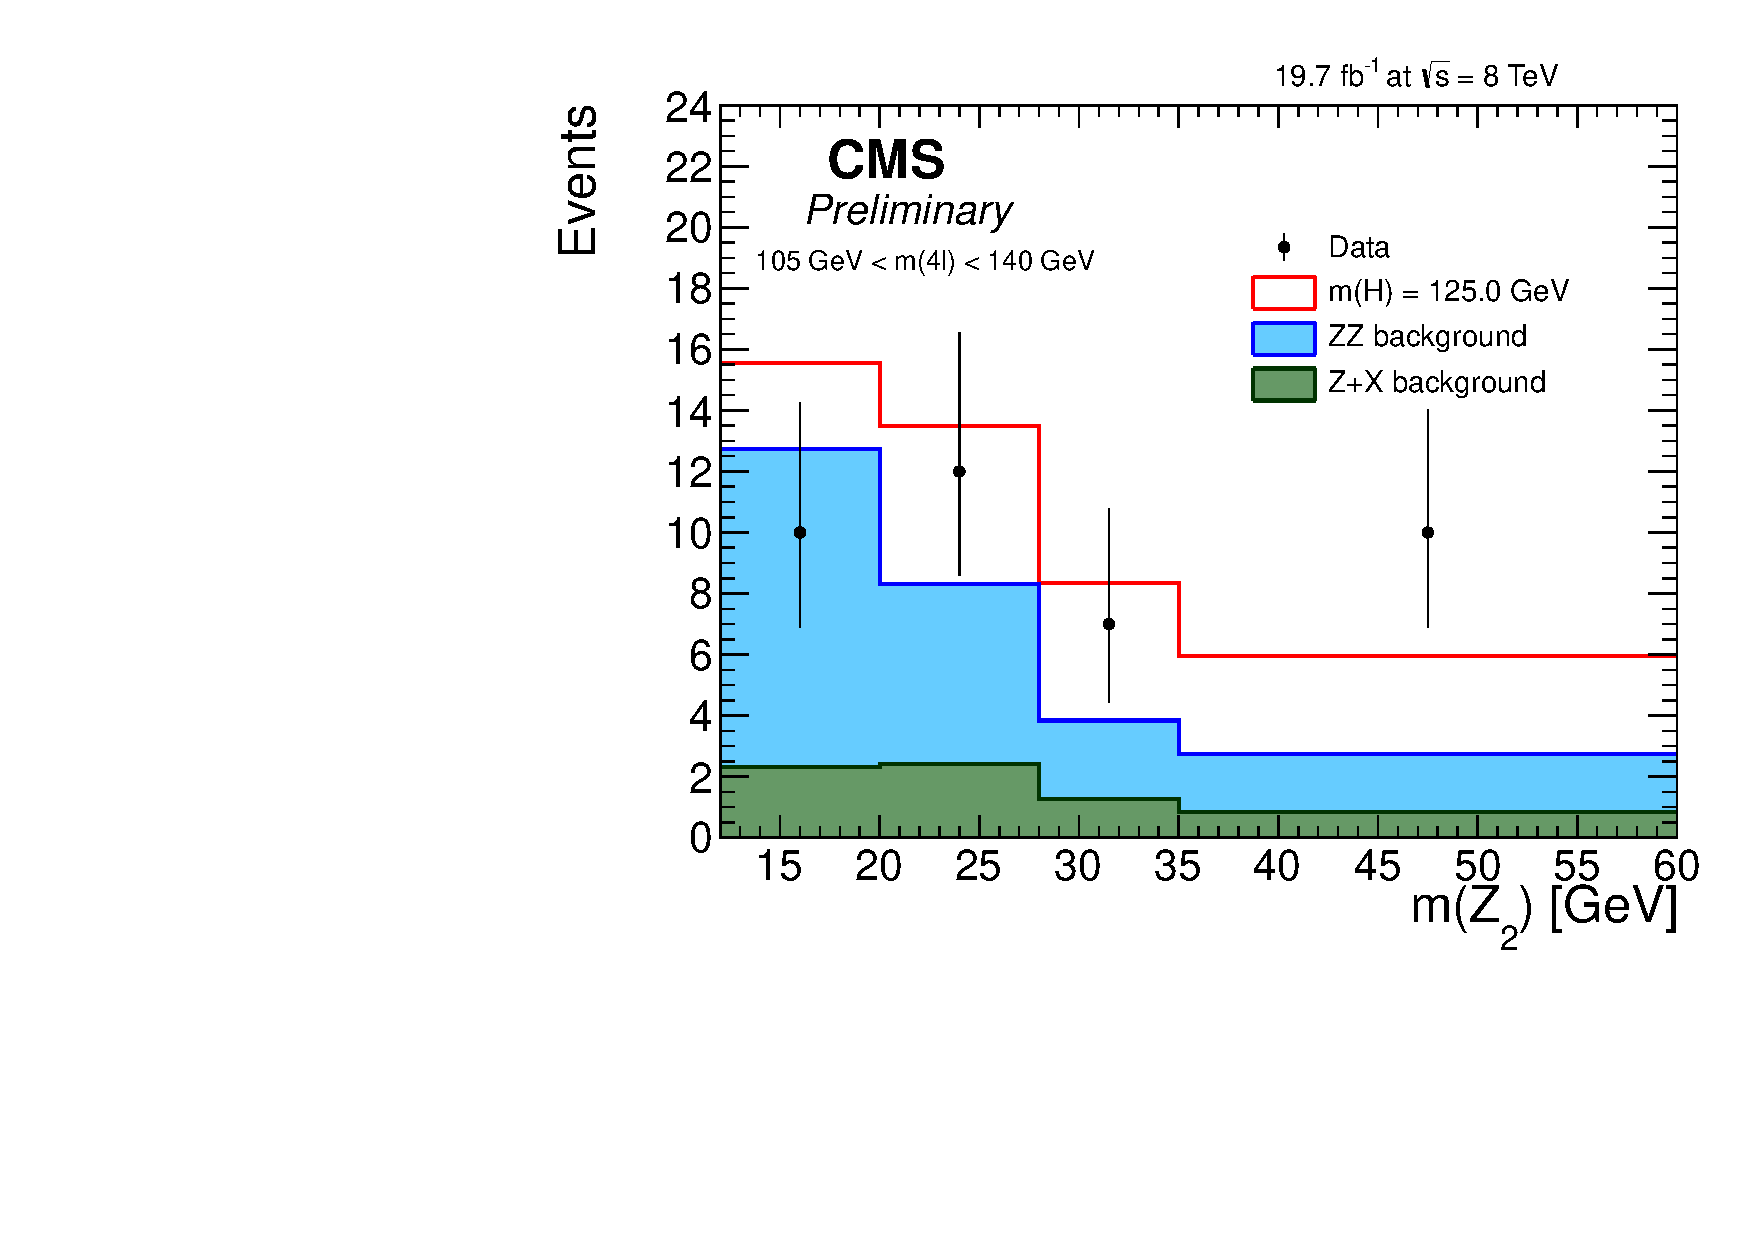
\includegraphics[width=0.33\textwidth,angle=0]{Plots/data_massZ2_4l.pdf}
      \label{fig:differential-bins:d}
    }
    \caption{Observed data along with the SM signal (m(H)=$125.0 \GeV$) and background expectations for different observables and for all final 
    \states combined, in range $105 < m_{4\ell} < 140 \GeV$ used for the $\Hllll$ measurements. The extraction of the signal is performed by
    exploiting the differences in the expected $m_{4\ell}$ spectra of the signal and background contributions in each bin of an observable.}
  \label{fig:differential-bins}
\end{center}
\end{figure}

\begin{figure}[!h!tb]
  \begin{center}
    \subfigure[$|\cos \theta^{*}|$]{
      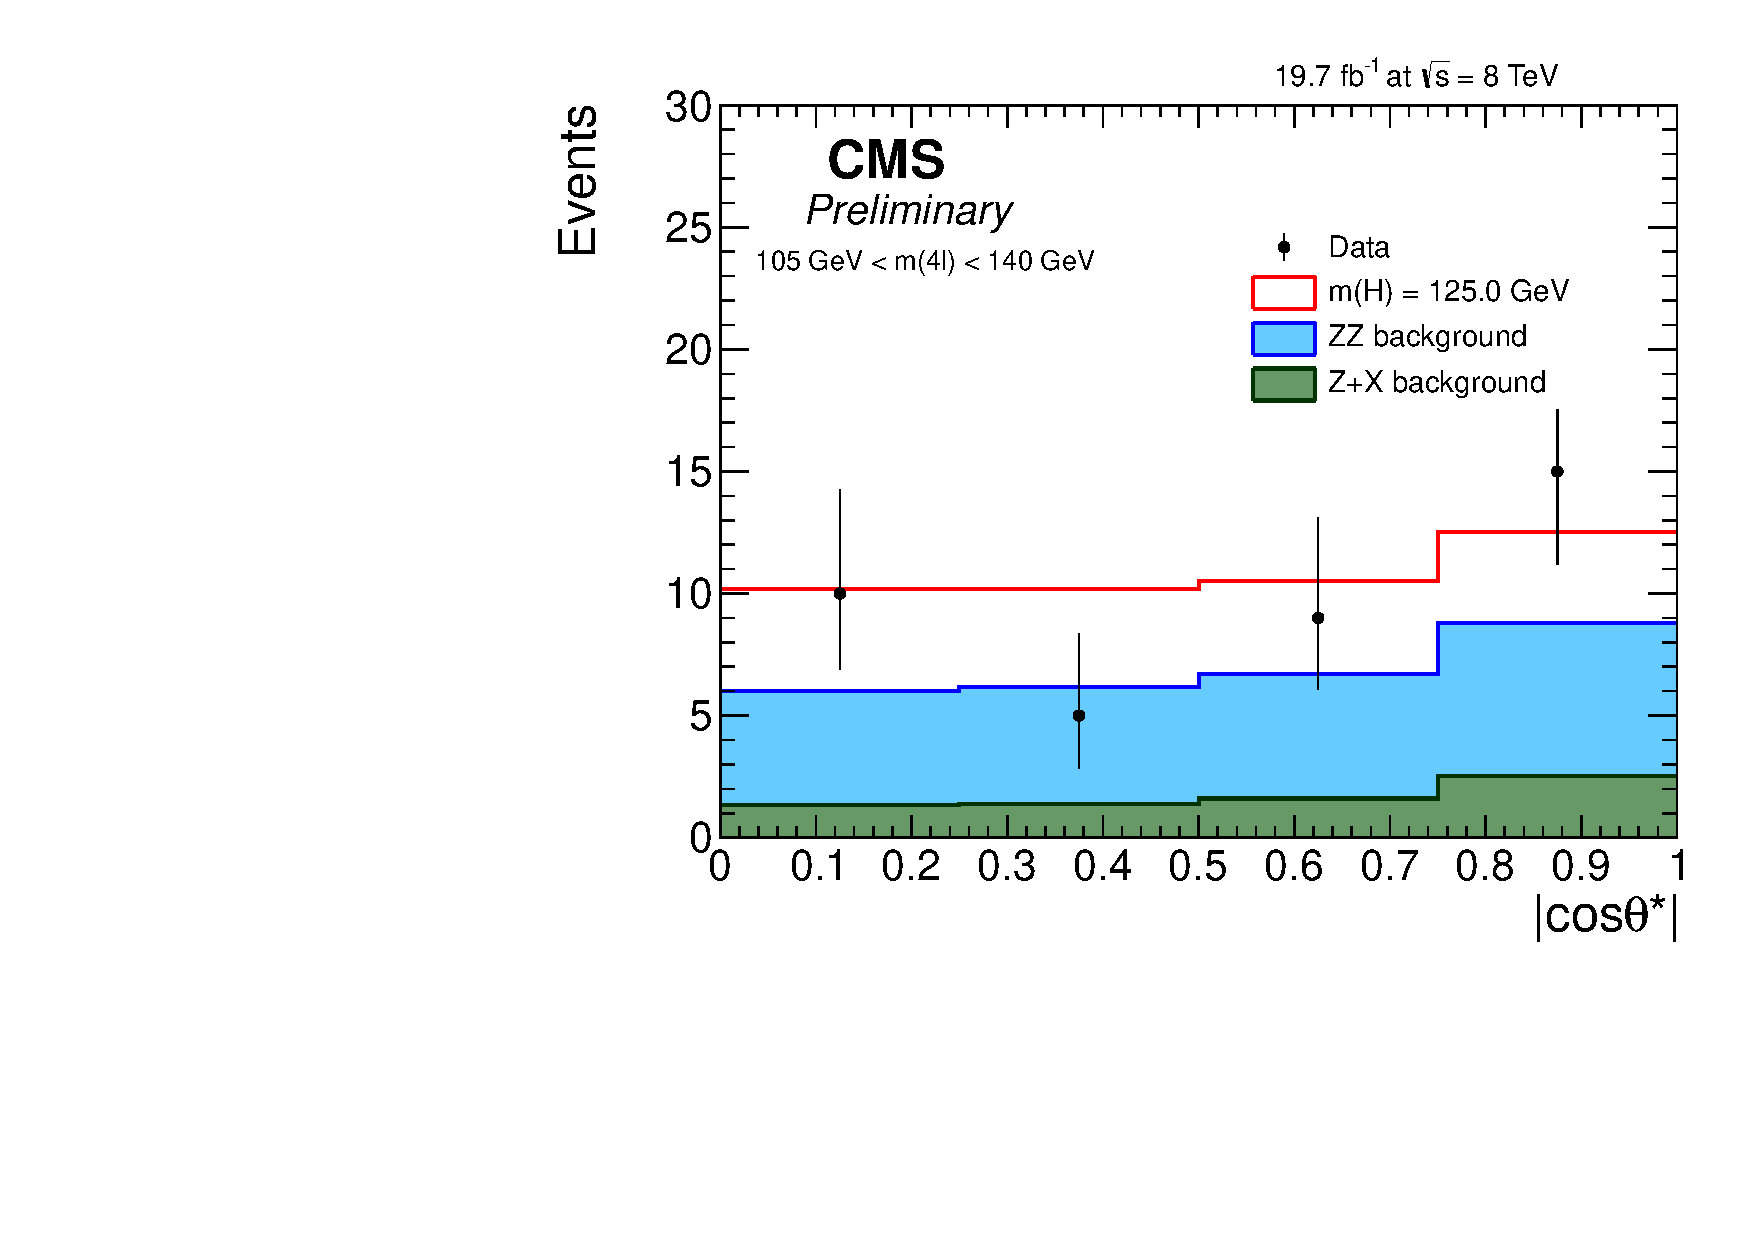
\includegraphics[width=0.33\textwidth,angle=0]{Plots/data_cosThetaStar_4l.pdf}
      \label{fig:differential-bins-2:a}
    }
    \subfigure[$|\cos \theta_{1}|$]{
      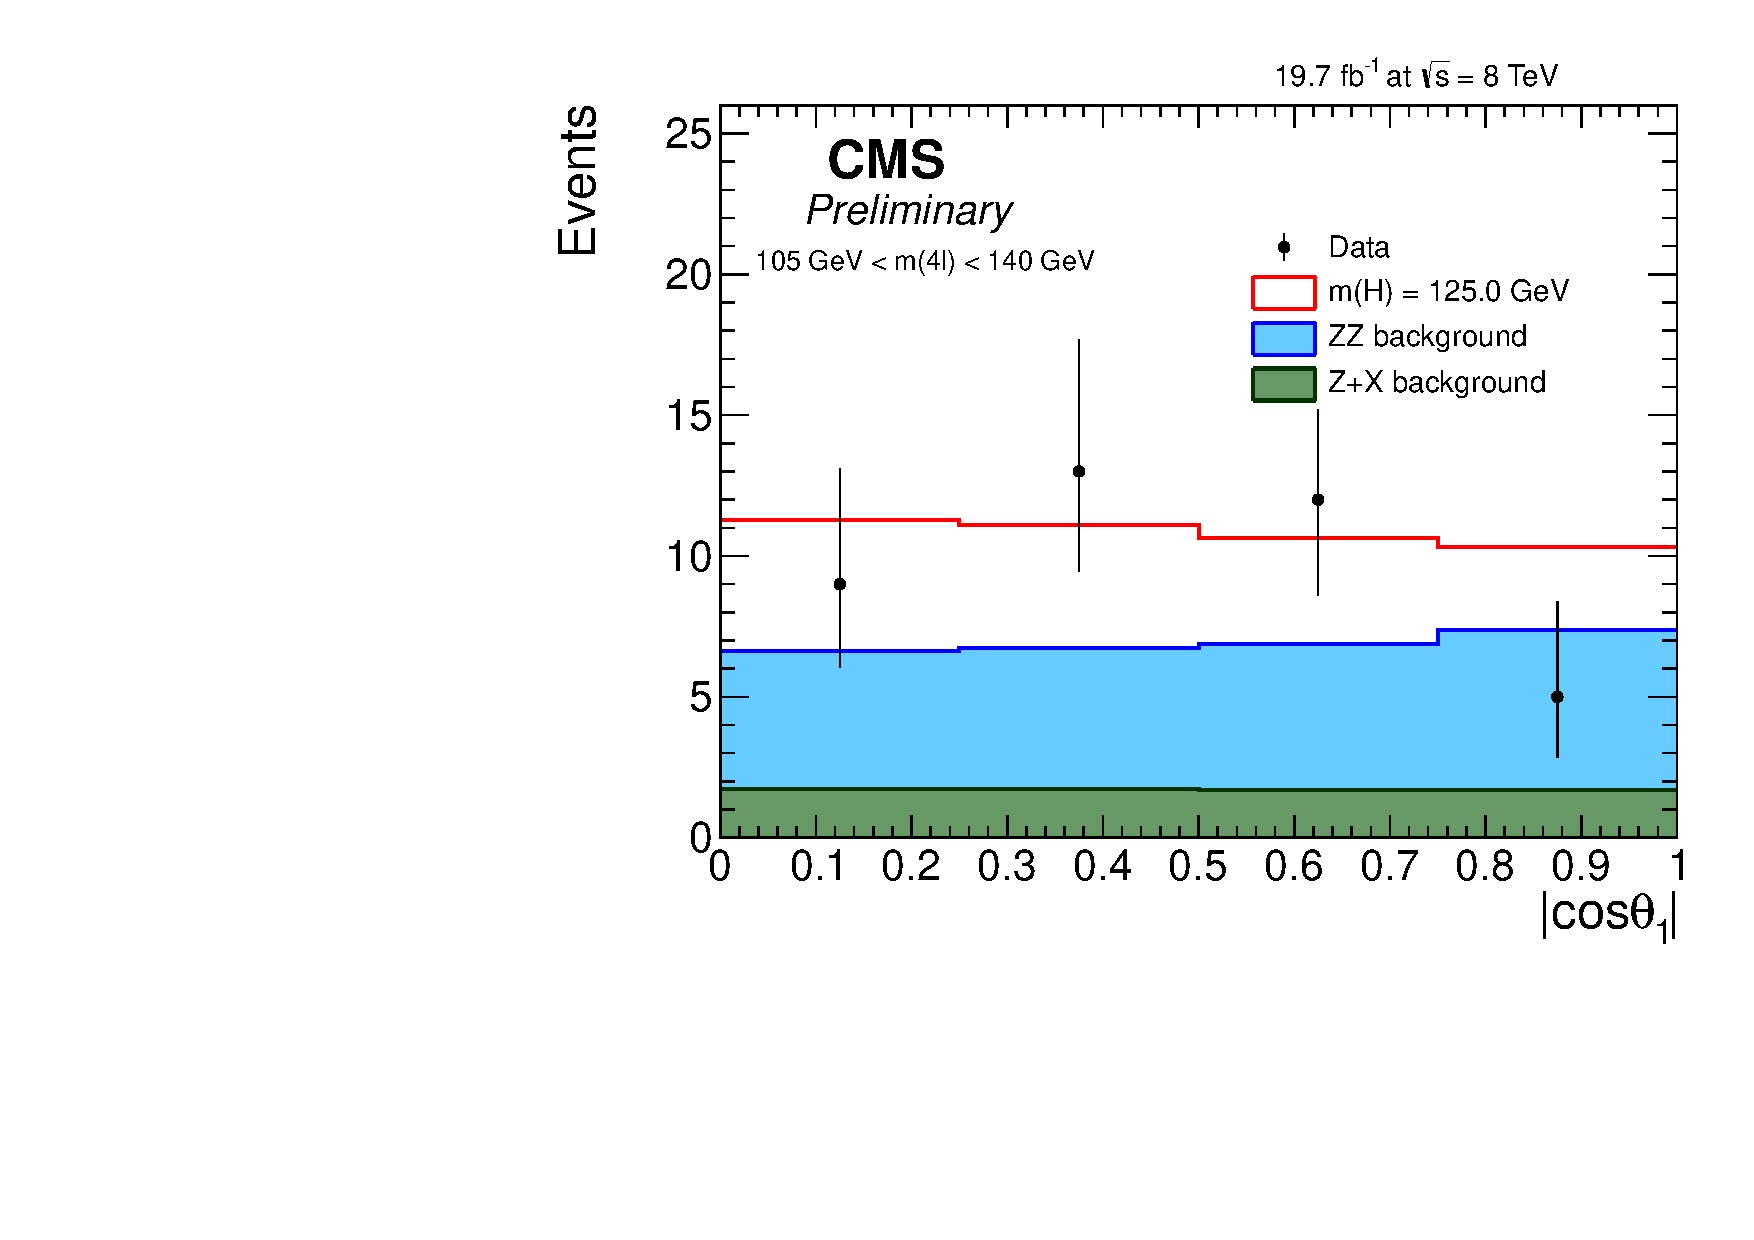
\includegraphics[width=0.33\textwidth,angle=0]{Plots/data_cosTheta1_4l.pdf}
      \label{fig:differential-bins-2:b}
    }
    \subfigure[$|\cos \theta_{2}|$]{
      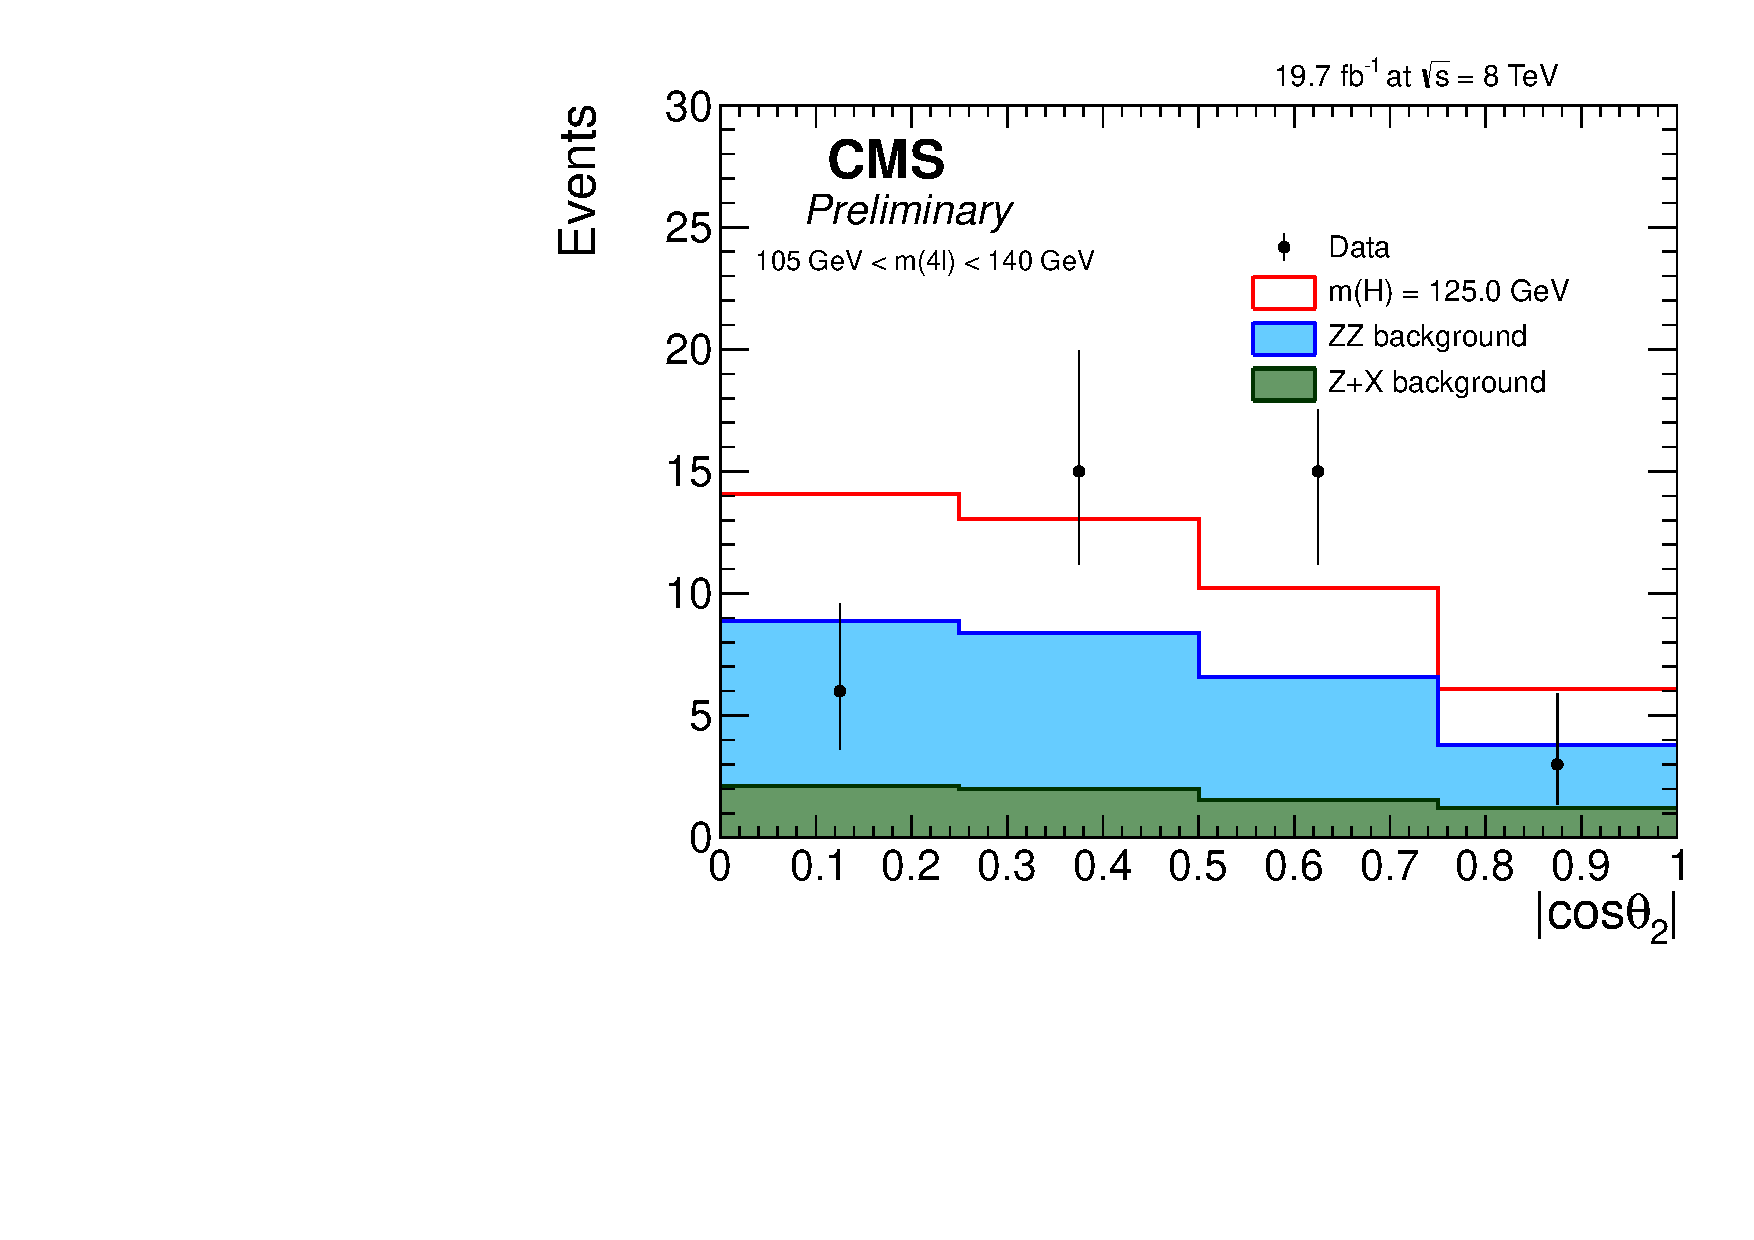
\includegraphics[width=0.33\textwidth,angle=0]{Plots/data_cosTheta2_4l.pdf}
      \label{fig:differential-bins-2:c}
    } \\
    \subfigure[$|\Phi|$]{
      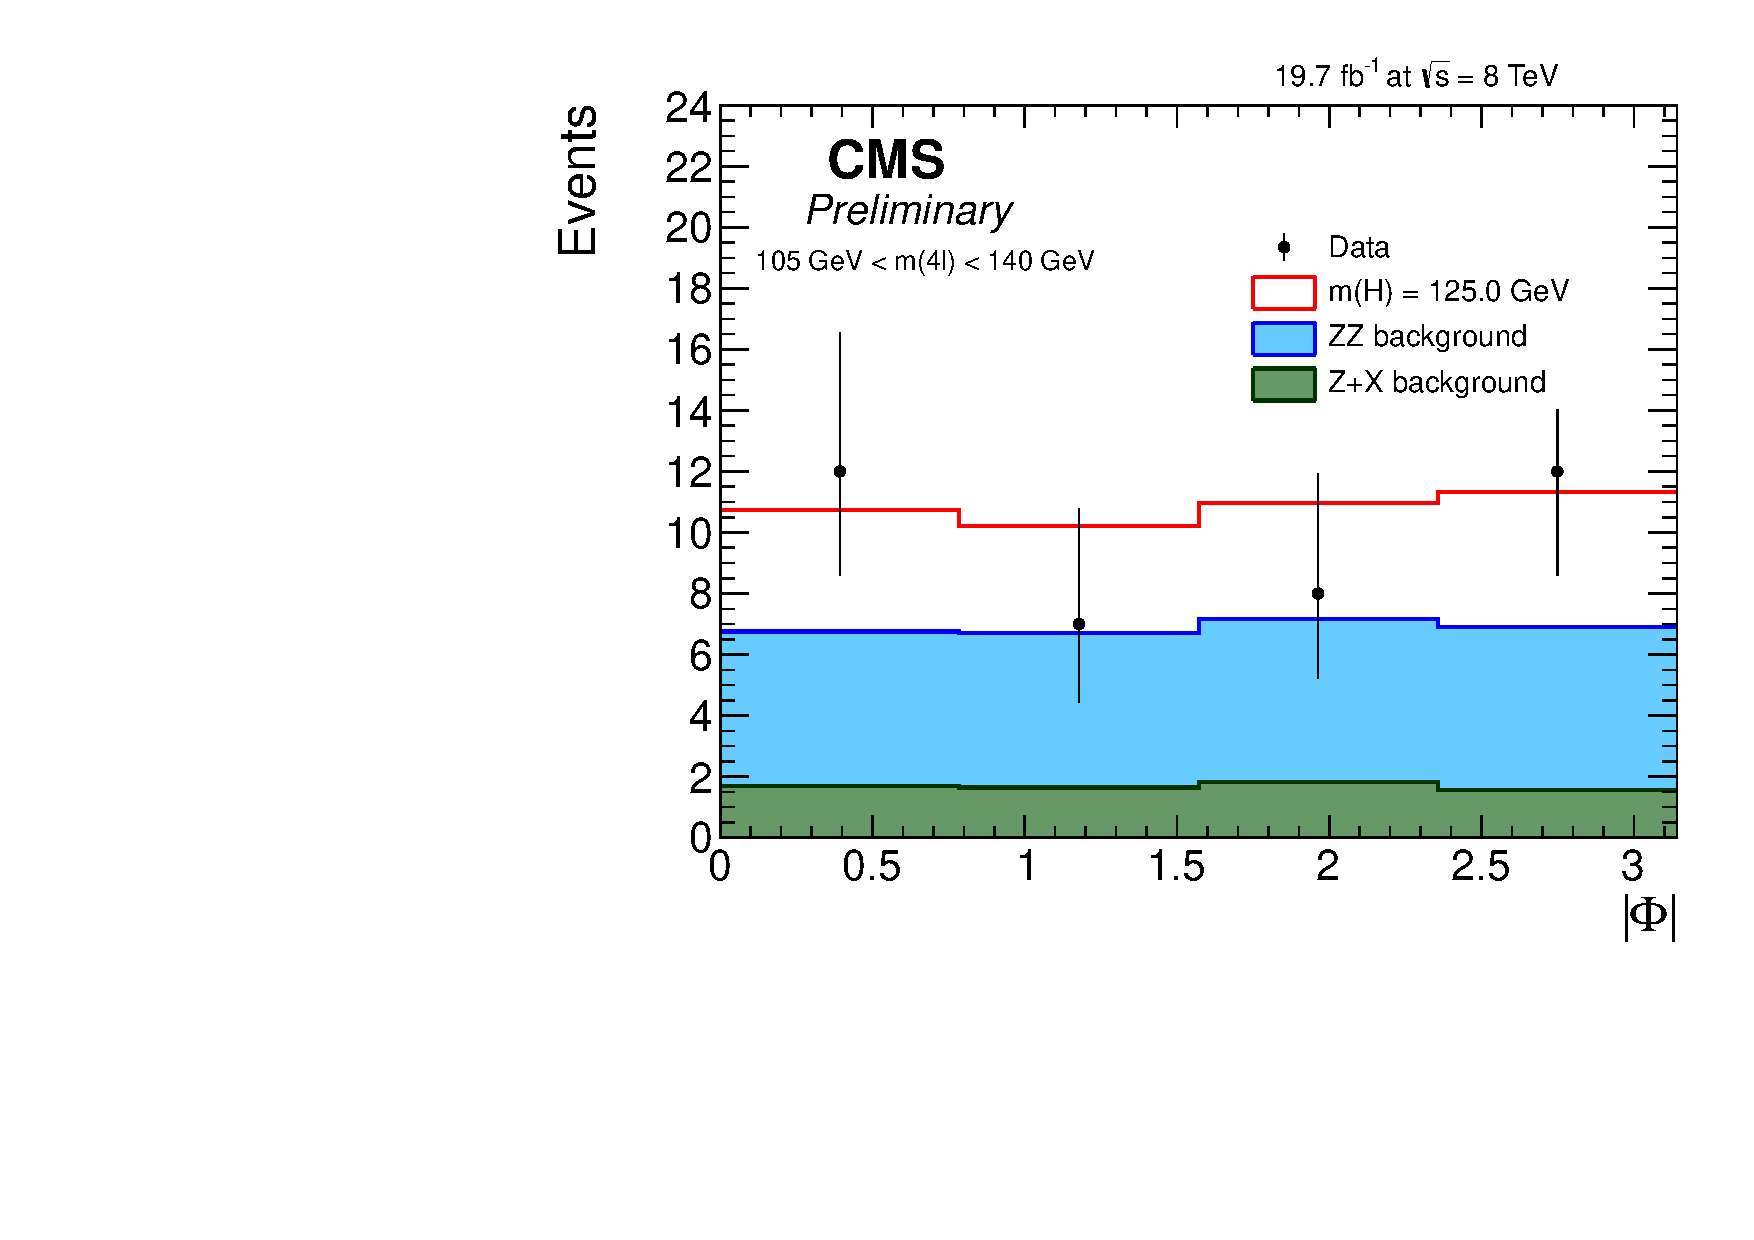
\includegraphics[width=0.33\textwidth,angle=0]{Plots/data_Phi_4l.pdf}
      \label{fig:differential-bins-2:d}
    }
    \subfigure[$\Phi_{1}$]{
      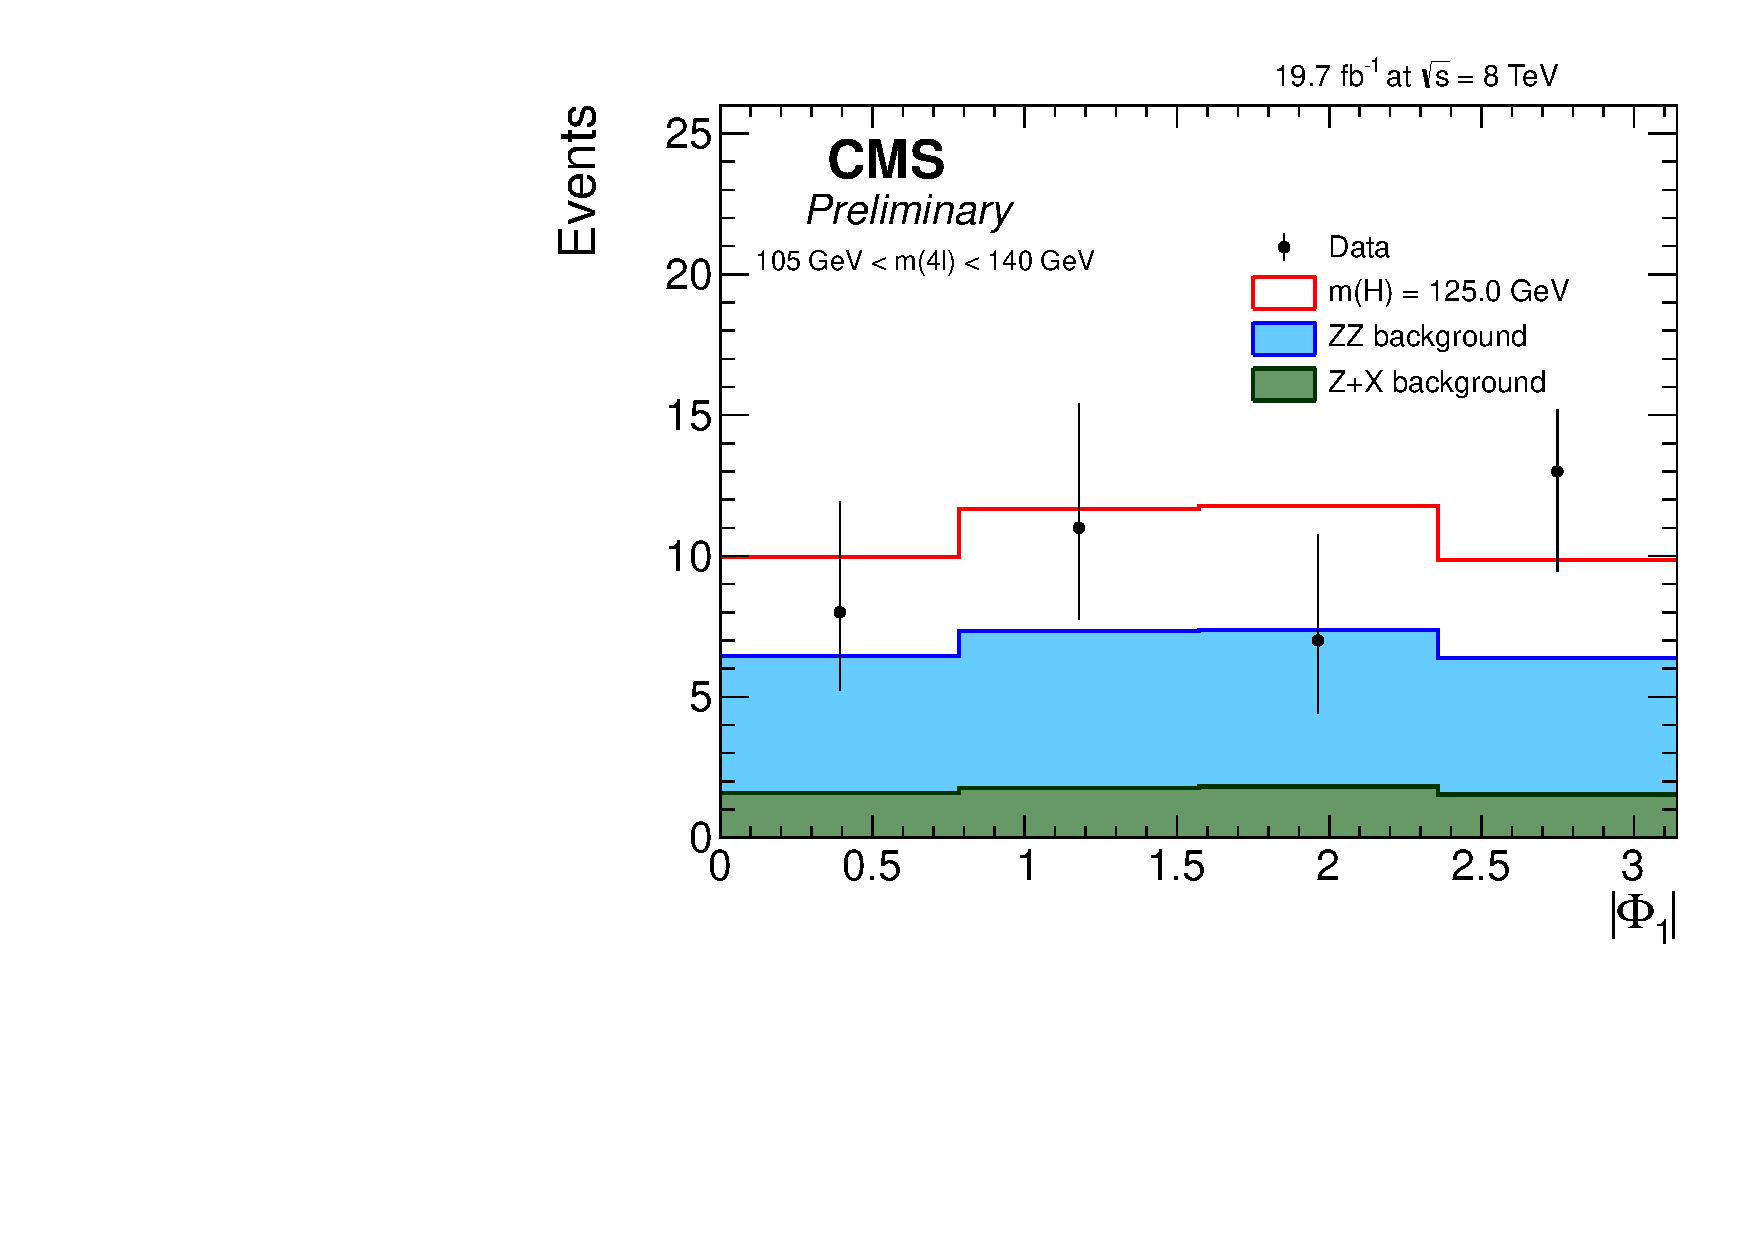
\includegraphics[width=0.33\textwidth,angle=0]{Plots/data_Phi1_4l.pdf}
      \label{fig:differential-bins-2:e}                             
    }\\
    \subfigure[$\mathrm{m}(\mathrm{Z}_{1})$]{
      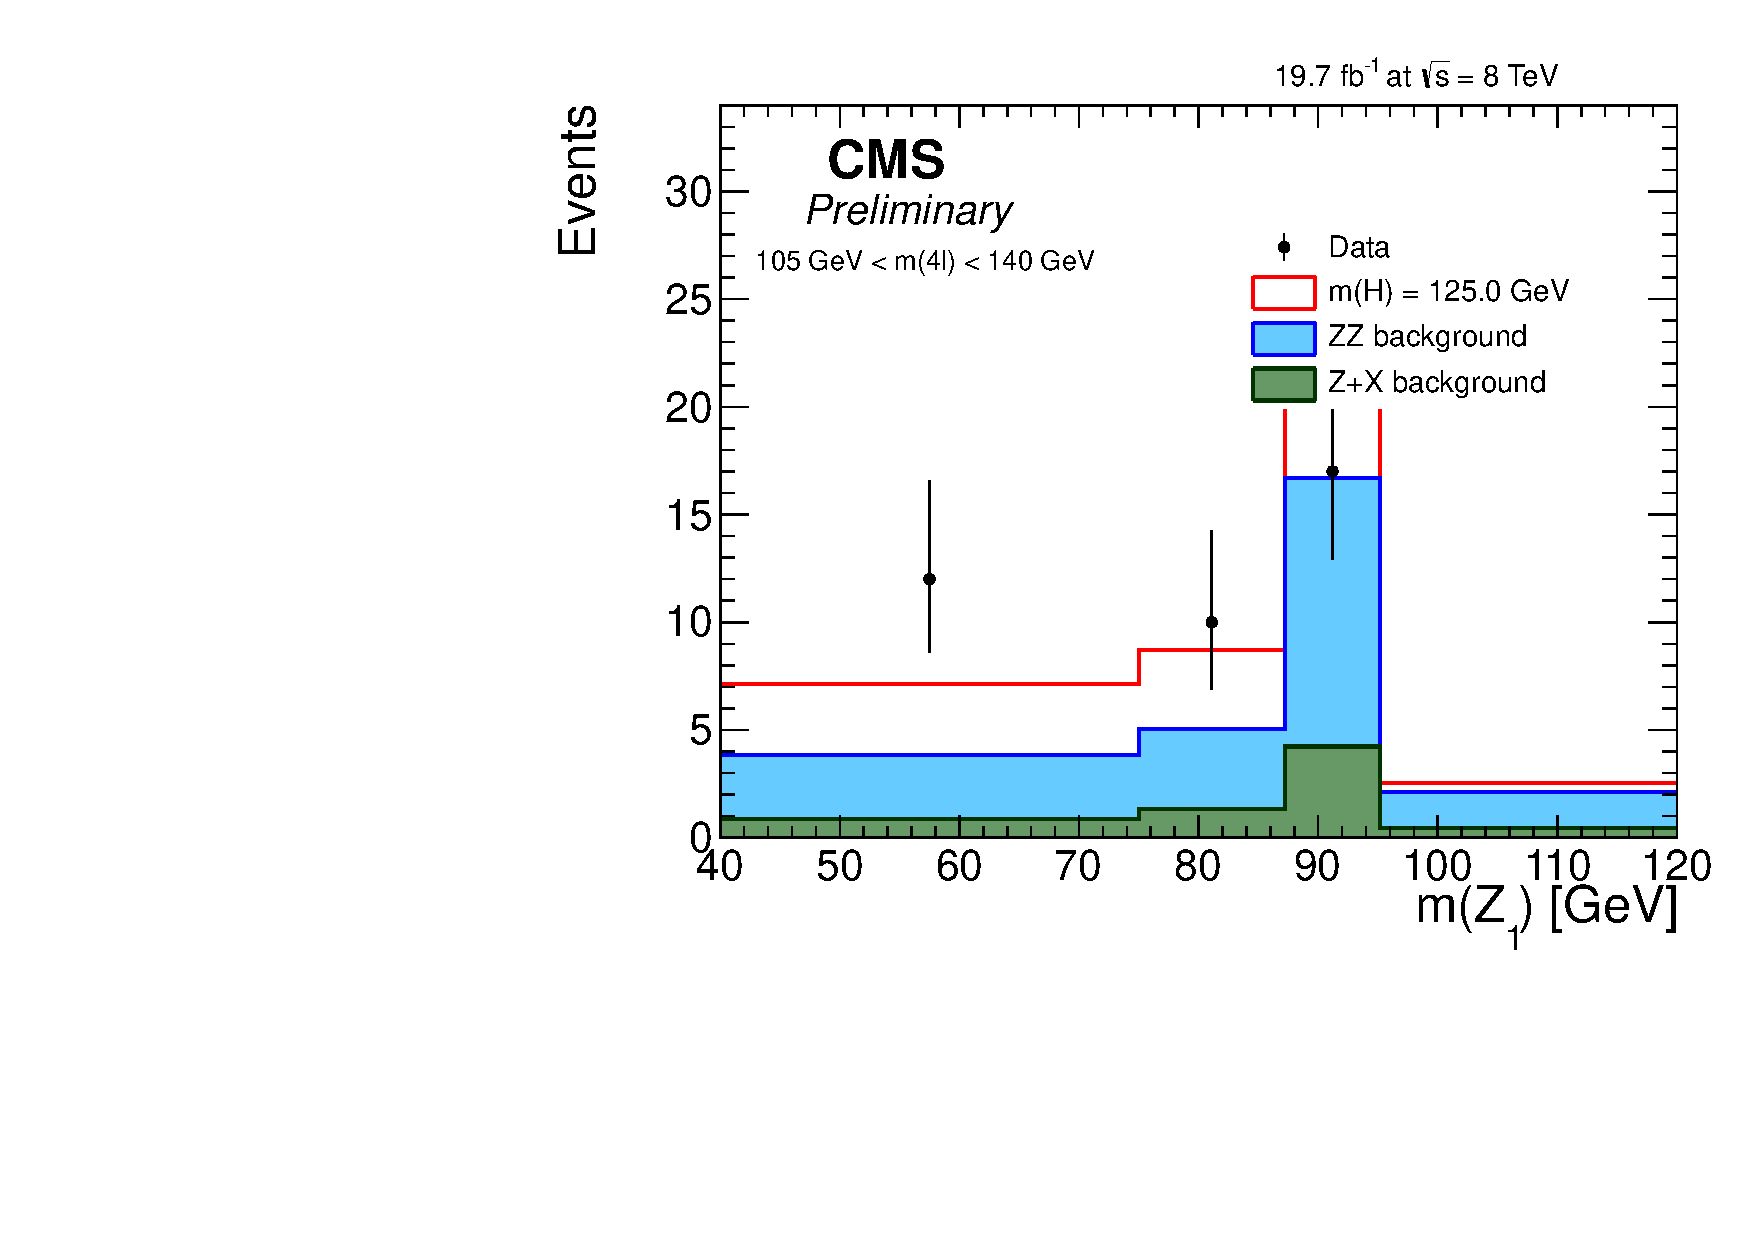
\includegraphics[width=0.33\textwidth,angle=0]{Plots/data_massZ1_4l.pdf}
      \label{fig:differential-bins:f}
    }
    \subfigure[$\mathrm{m}(\mathrm{Z}_{2})$]{
      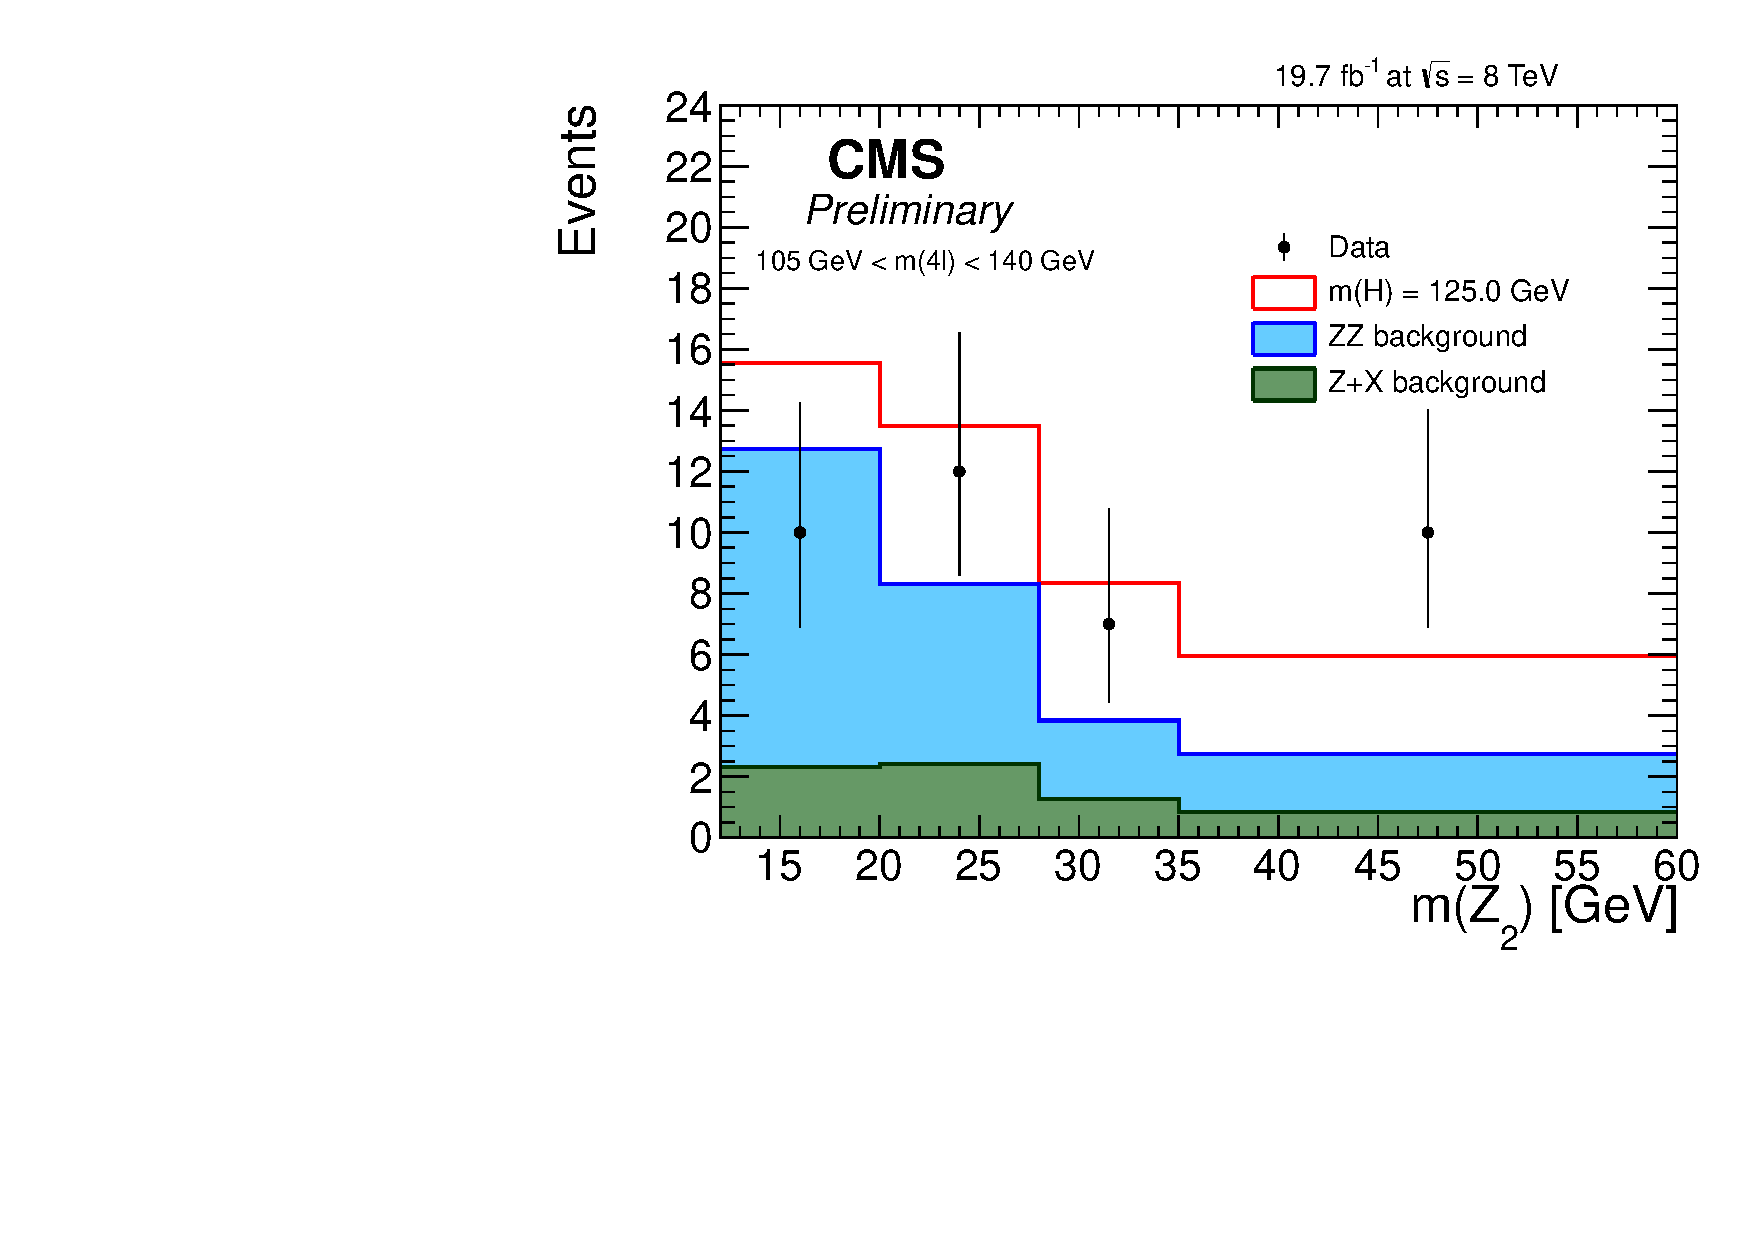
\includegraphics[width=0.33\textwidth,angle=0]{Plots/data_massZ2_4l.pdf}
      \label{fig:differential-bins:g}
    }
    \caption{Observed data along with the SM signal (m(H)=$125.0 \GeV$) and background expectations for different observables
    and for all final states combined, in range $105 < m_{4\ell} < 140 \GeV$ used for the $\Hllll$ measurements. The extraction of the 
    signal is performed by exploiting the differences in the expected $m_{4\ell}$ spectra of the signal and background contributions in
    each bin of an observable.
    }
  \label{fig:differential-bins-2}
 \end{center}
\end{figure}

\begin{figure}[!h!tb]
  \begin{center}
    \subfigure[$\pt(\mathrm{H})$]{
      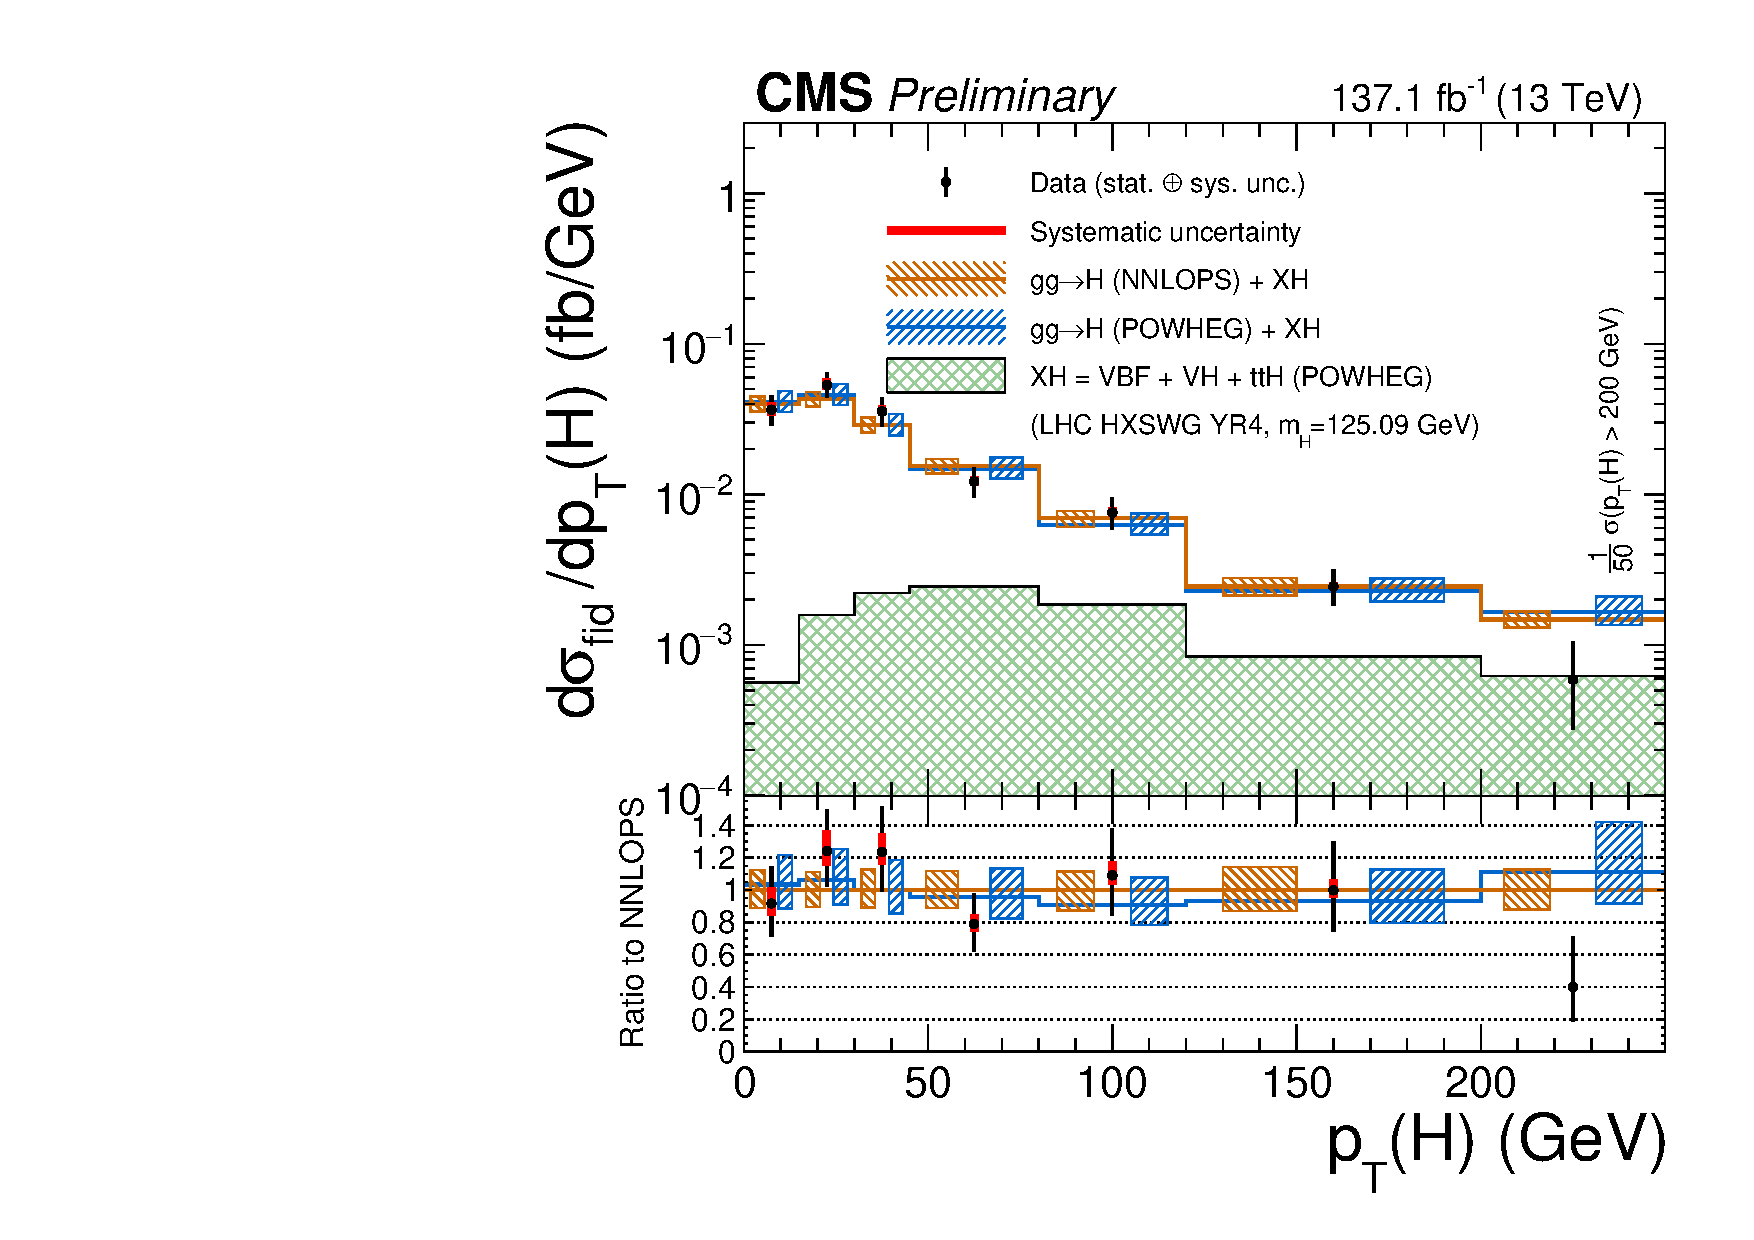
\includegraphics[width=0.40\textwidth,angle=0]{Plots/pT4l_unfoldwith_SM_125_logscale.pdf}
      \label{fig:differential-results:a}
    }
    \subfigure[$|y(\mathrm{H})|$]{
      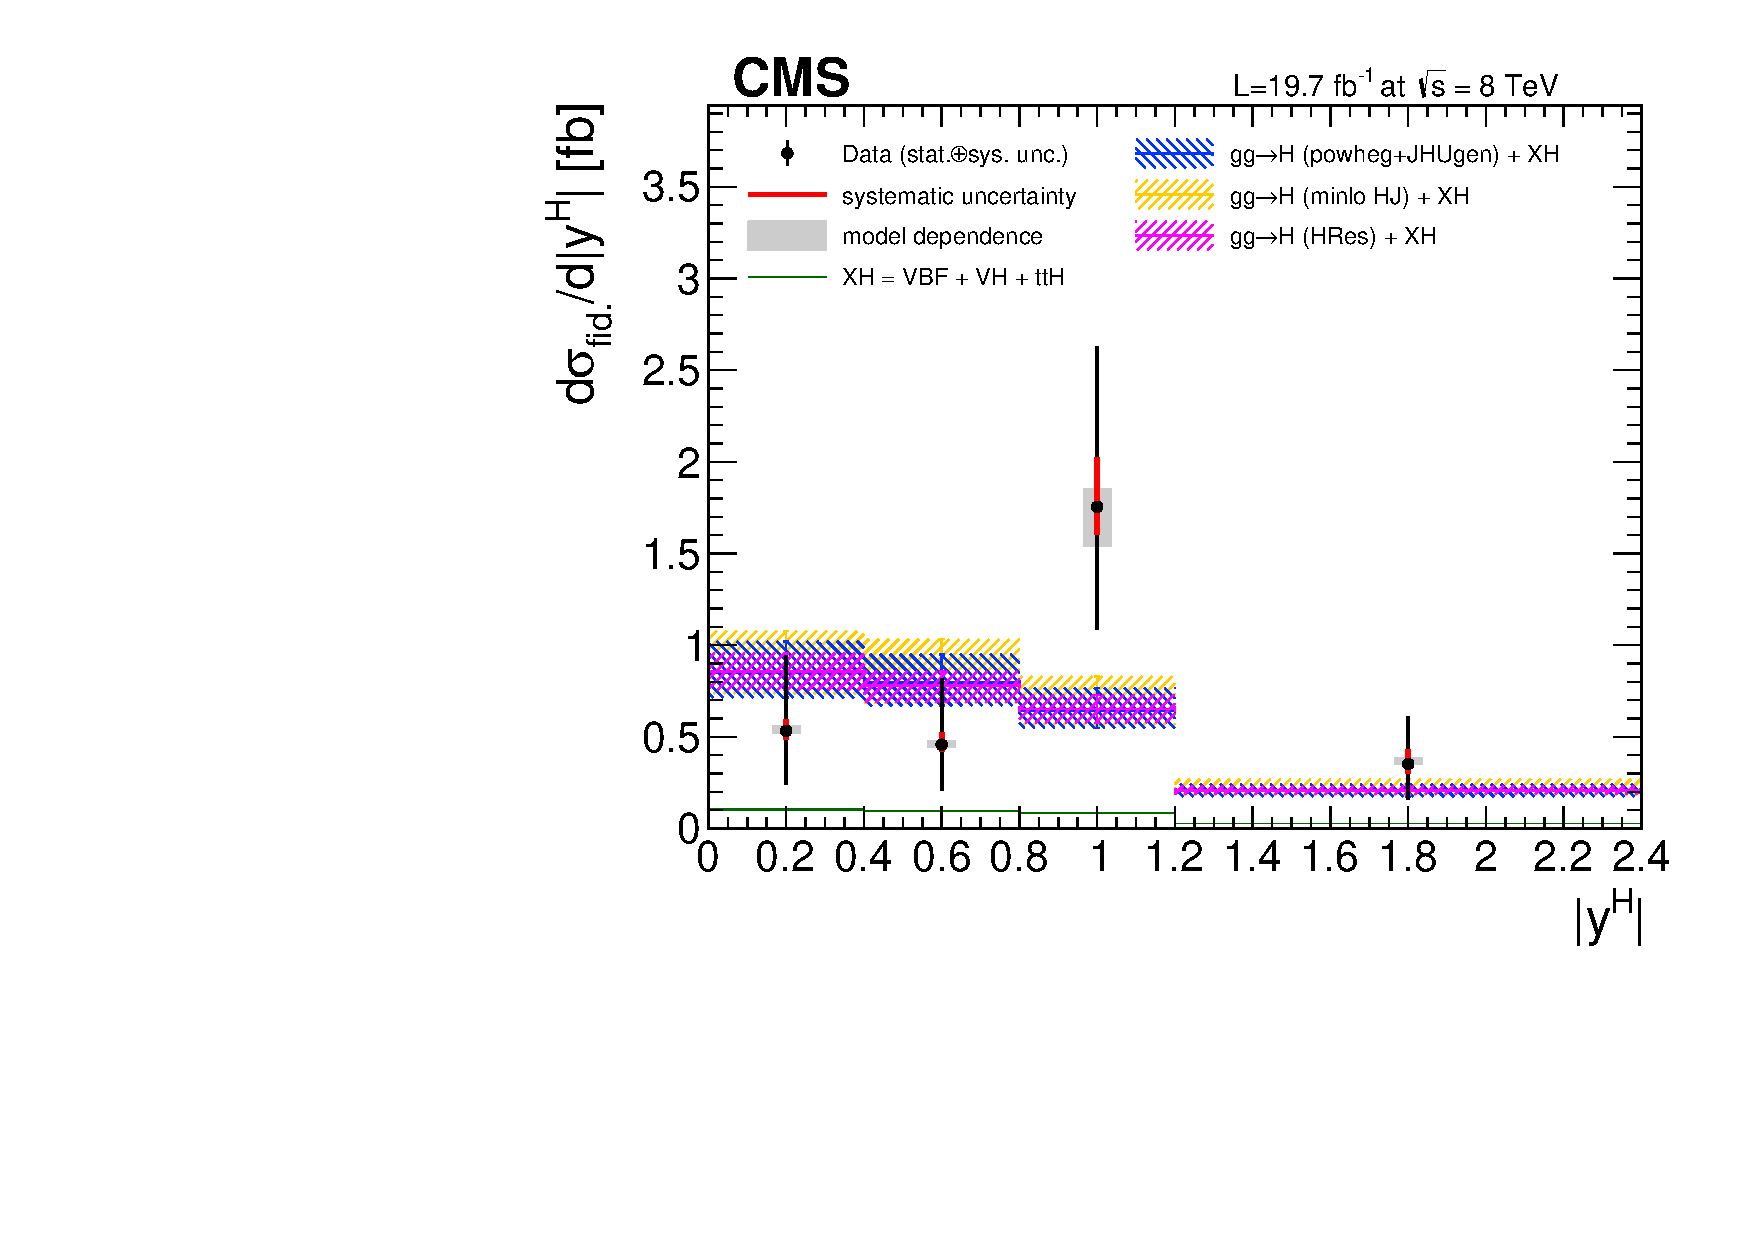
\includegraphics[width=0.40\textwidth,angle=0]{Plots/rapidity4l_unfoldwith_SM_125.pdf}
      \label{fig:differential-results:b}
    } \\
    \subfigure[$\pt(\mathrm{leading~jet})$]{
      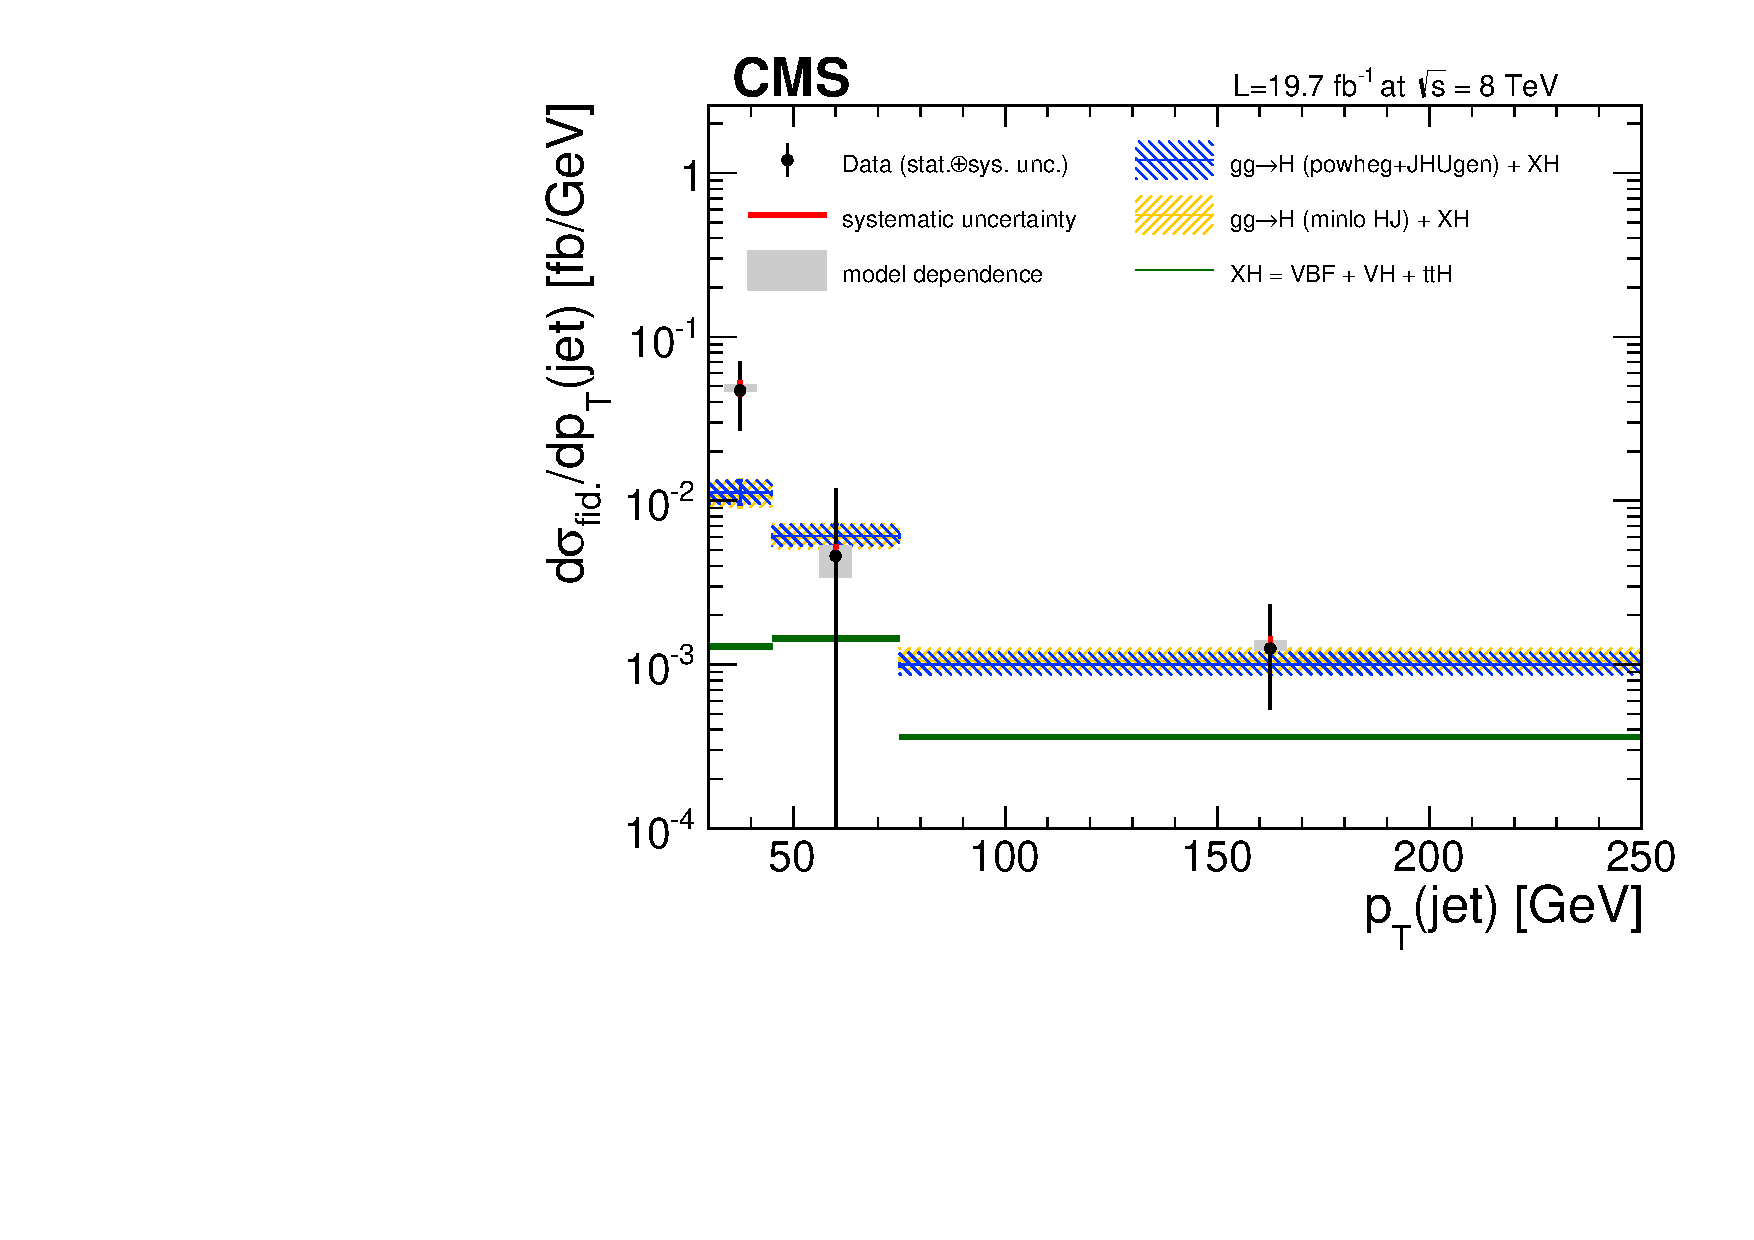
\includegraphics[width=0.40\textwidth,angle=0]{Plots/pt_leadingjet_reco_pt30_eta4p7_unfoldwith_SM_125_logscale.pdf}
      \label{fig:differential-results:c}
    }
    \subfigure[$|y(\mathrm{H}) - y(\mathrm{leading~jet})|$]{
      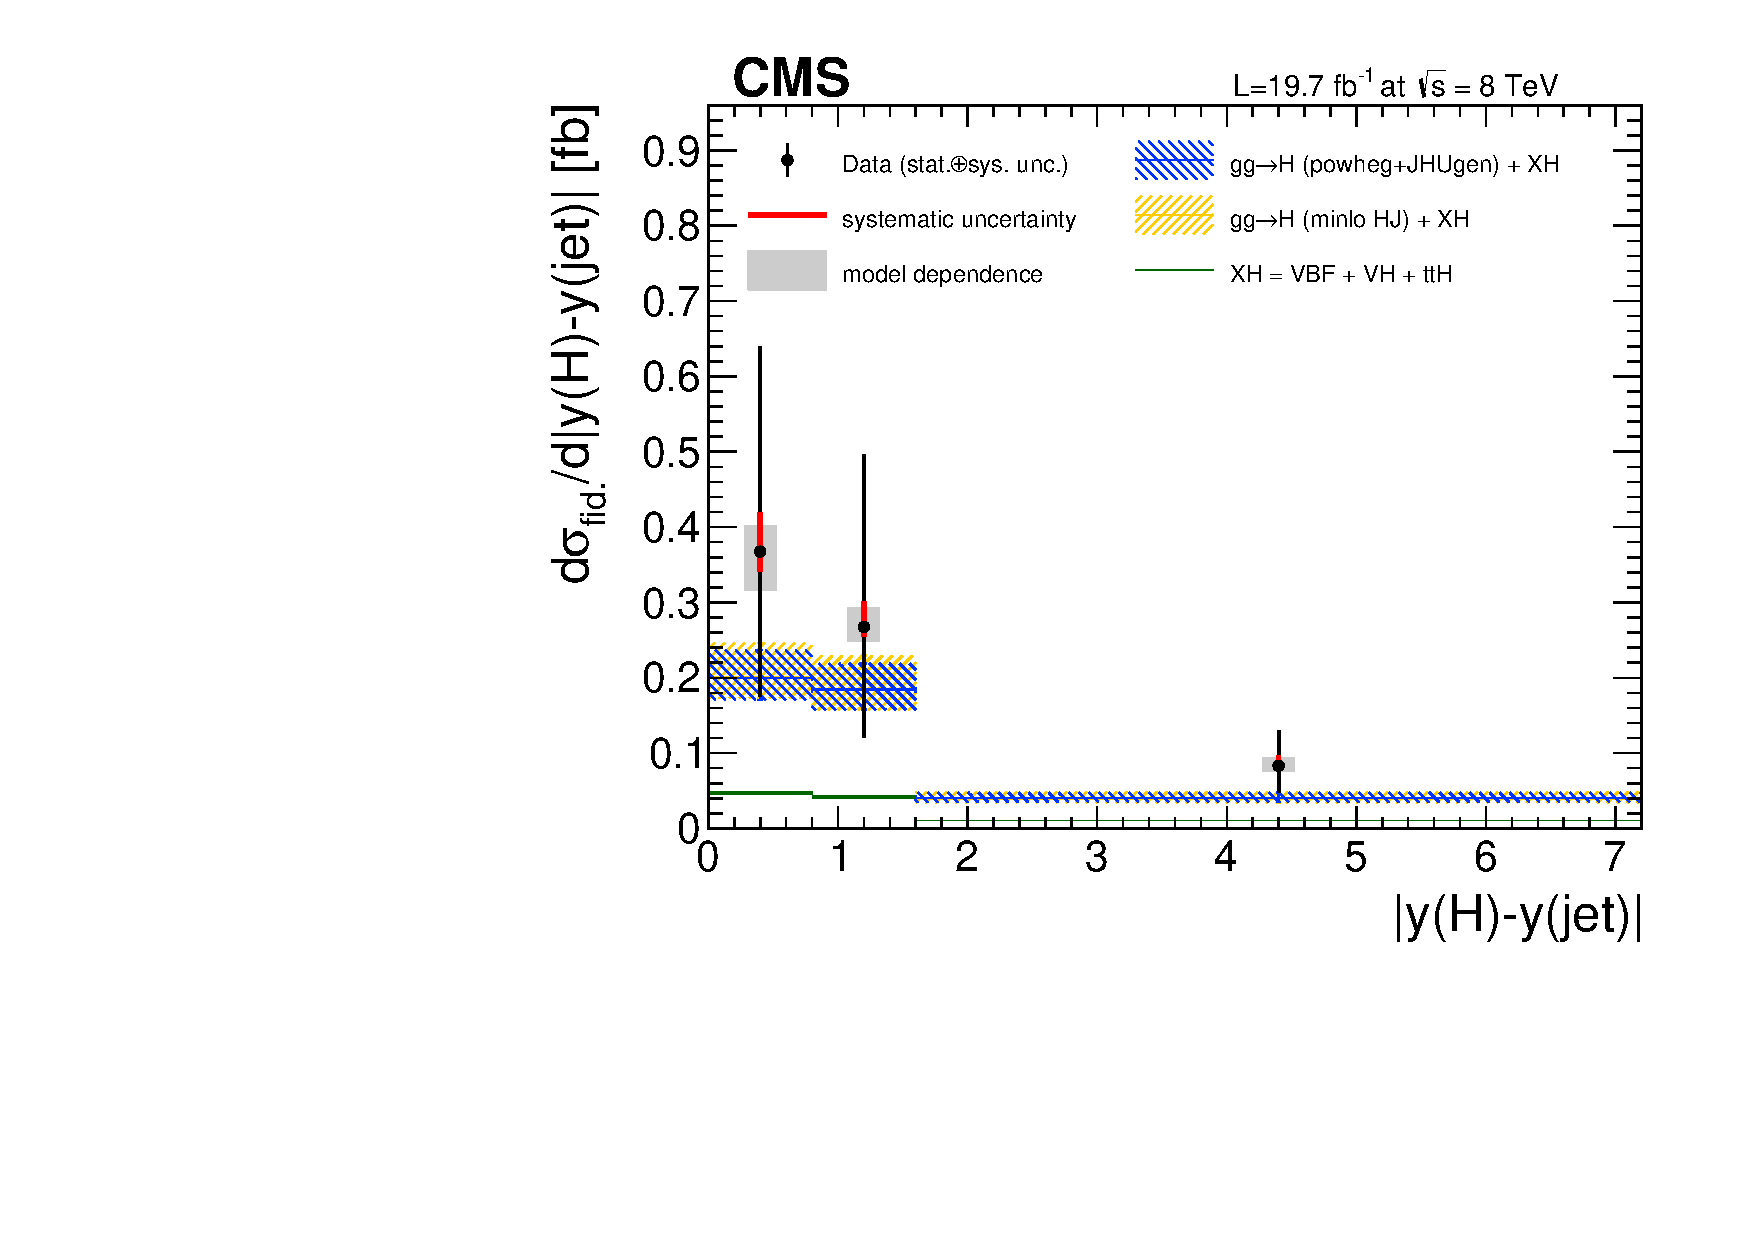
\includegraphics[width=0.40\textwidth,angle=0]{Plots/absdeltarapidity_hleadingjet_reco_pt30_eta4p7_unfoldwith_SM_125.pdf}
      \label{fig:differential-results:d}
    } \\
    \subfigure[N(jets), $|\eta|<4.7$]{
      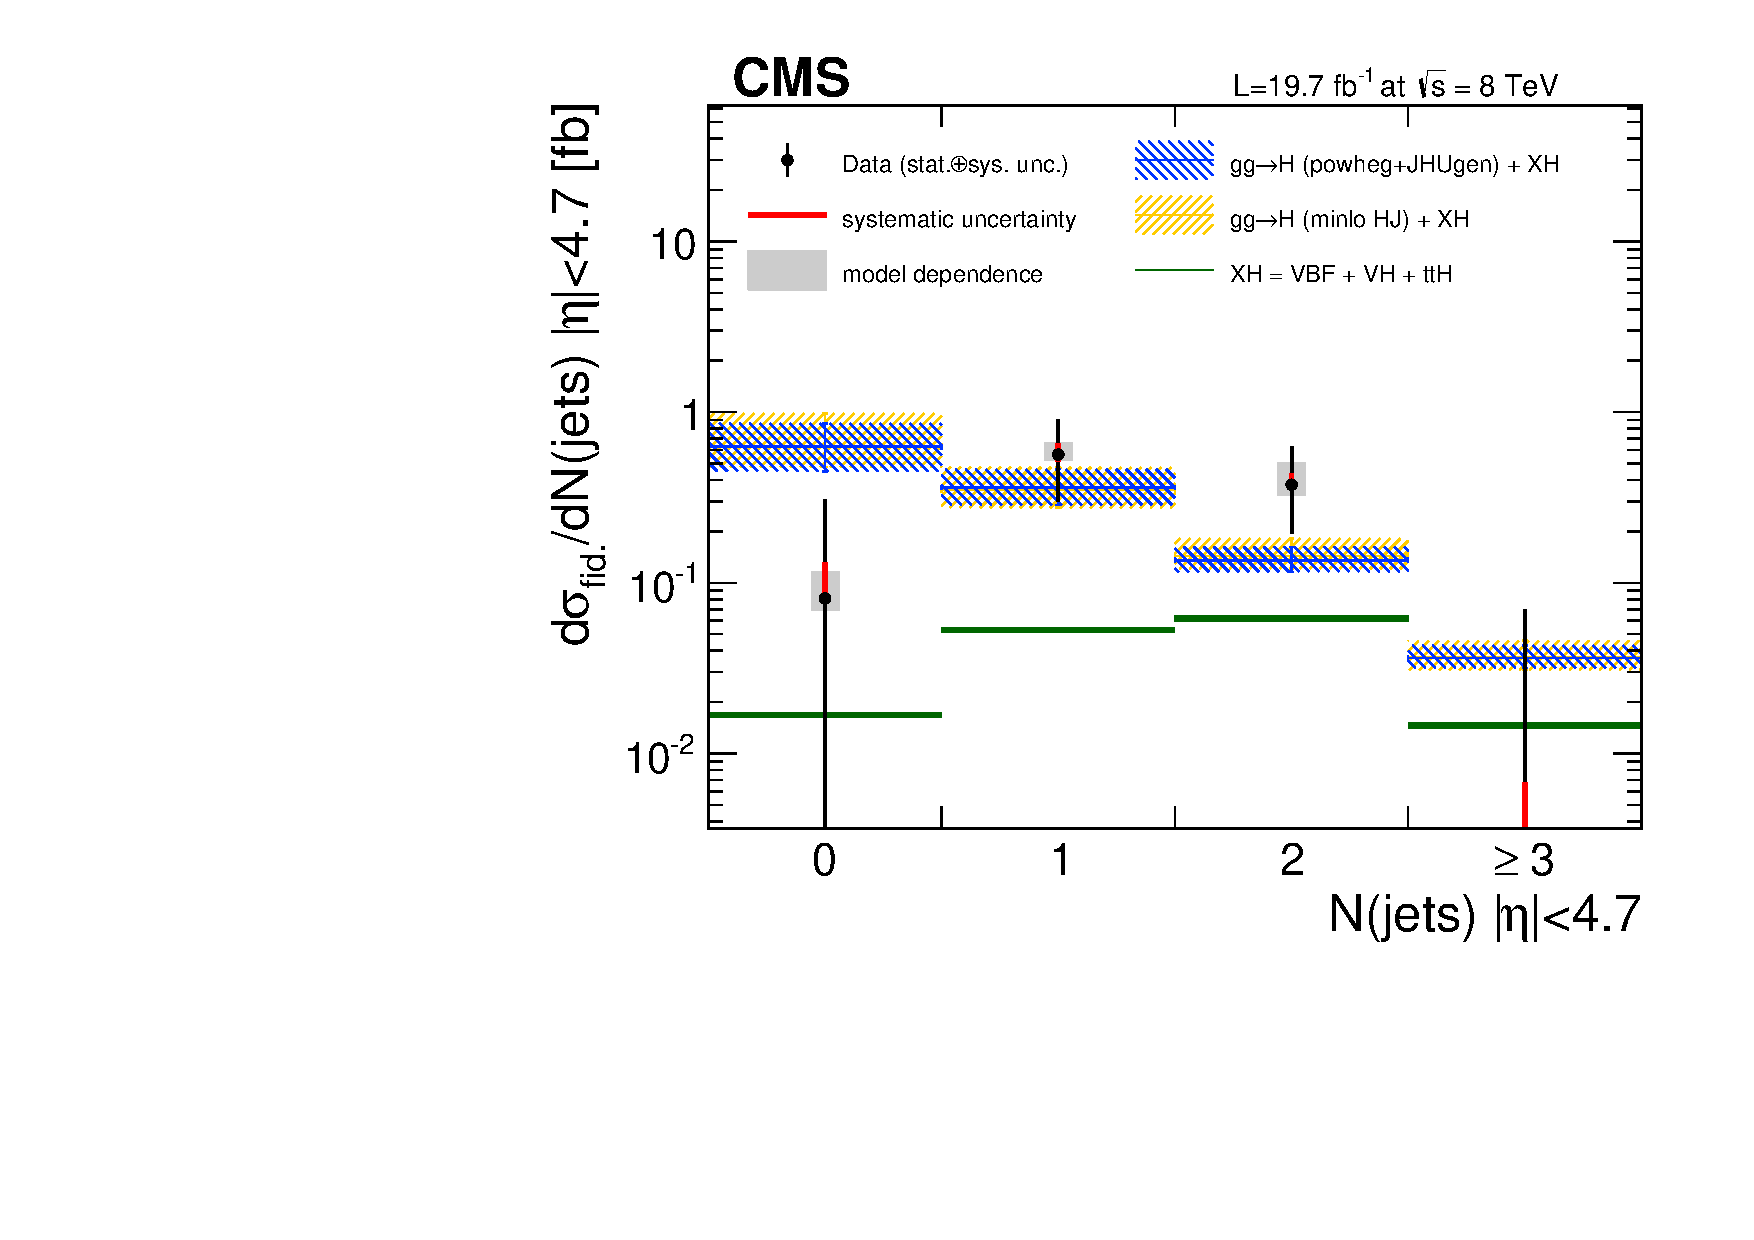
\includegraphics[width=0.40\textwidth,angle=0]{Plots/njets_reco_pt30_eta4p7_unfoldwith_SM_125_logscale.pdf}
      \label{fig:differential-results:e}
    } 
    \subfigure[N(jets), $|\eta|<2.5$]{
      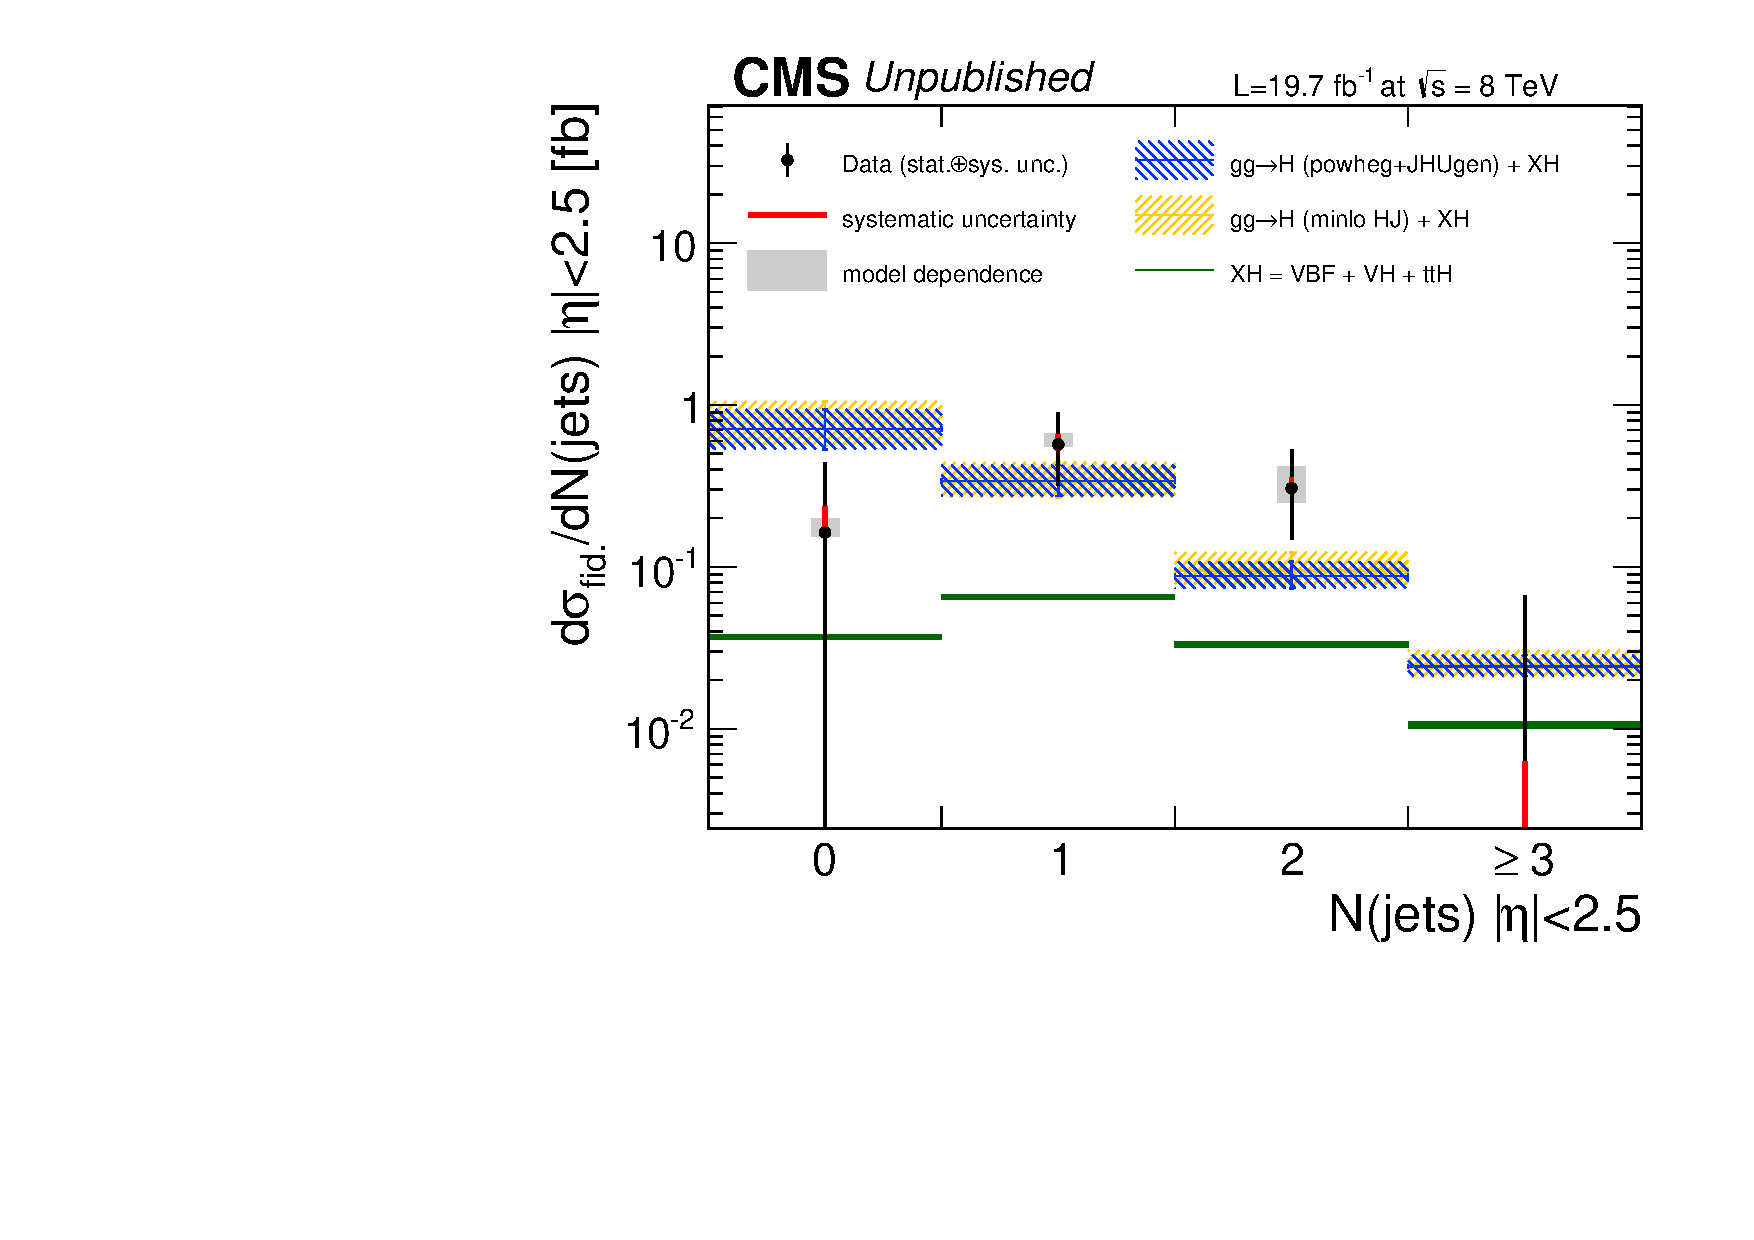
\includegraphics[width=0.40\textwidth,angle=0]{Plots/njets_reco_pt30_eta2p5_unfoldwith_SM_125_logscale_unpublished.pdf}
      \label{fig:differential-results:f}
    }
    \caption{The differential fiducial cross section results of $\Hllll$ and comparison with the theoretical pridictions. 
        Systematic uncertainty is indicated by red bars while black bars shows the total statistical and systematic uncertainties, combined in quadrature.
        The model dependence is shown as an additional systematic uncertainty by the grey boxes.  The pink, yellow and blue colors shows
        the theoretical predictions, where acceptance of the 
        dominant $\ggH$ production mode is calculated by {\sc HRes},{\sc powheg minlo-HJ}+{\sc Pythia} and  {\sc powheg+JHUgen}+{\sc Pythia} respectively.
        The sub-dominant production contributions XH $=$ VBF $+$ VH $+$ $\ttH$ are shown in green separately. The total inclusive cross section is 
        normalized to the SM estimate computed at NNLL+NNLO accuracy for all theoretical predictions. The systematic uncertainties correspond to the 
        generators accuracy are also taken in to account for differential predictions. The fraction of $4e,4\mu$ and $2e2\mu$ in each bin is allowed 
        to float in the fit.
    }
  \label{fig:differential-results}
 \end{center}
\end{figure}

\begin{figure}[!h!tb]
  \begin{center}
    \subfigure[$|\cos \theta^{*}|$]{
      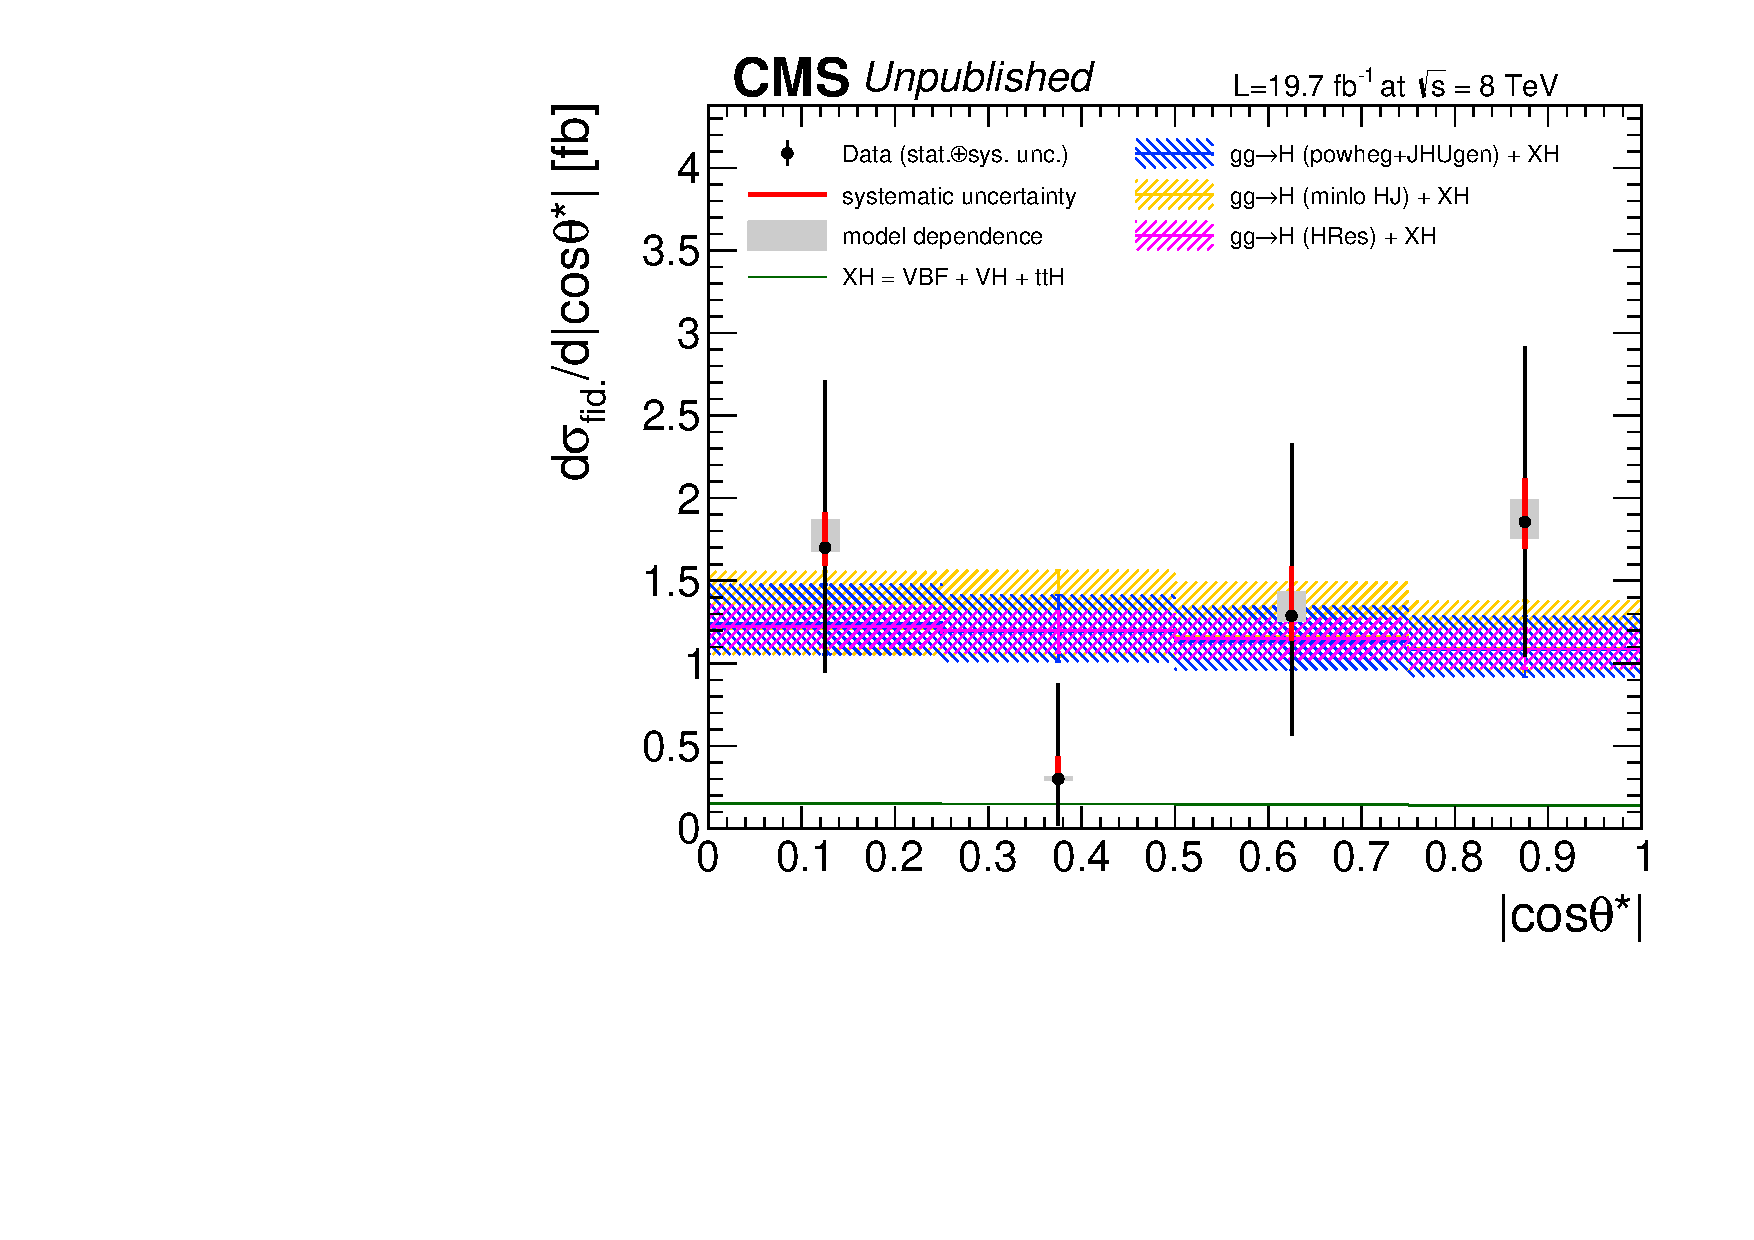
\includegraphics[width=0.30\textwidth,angle=0]{Plots/cosThetaStar_unfoldwith_SM_125_unpublished.pdf}
      \label{fig:differential-results-2:a}
    }
    \subfigure[$|\cos \theta_{1}|$]{
      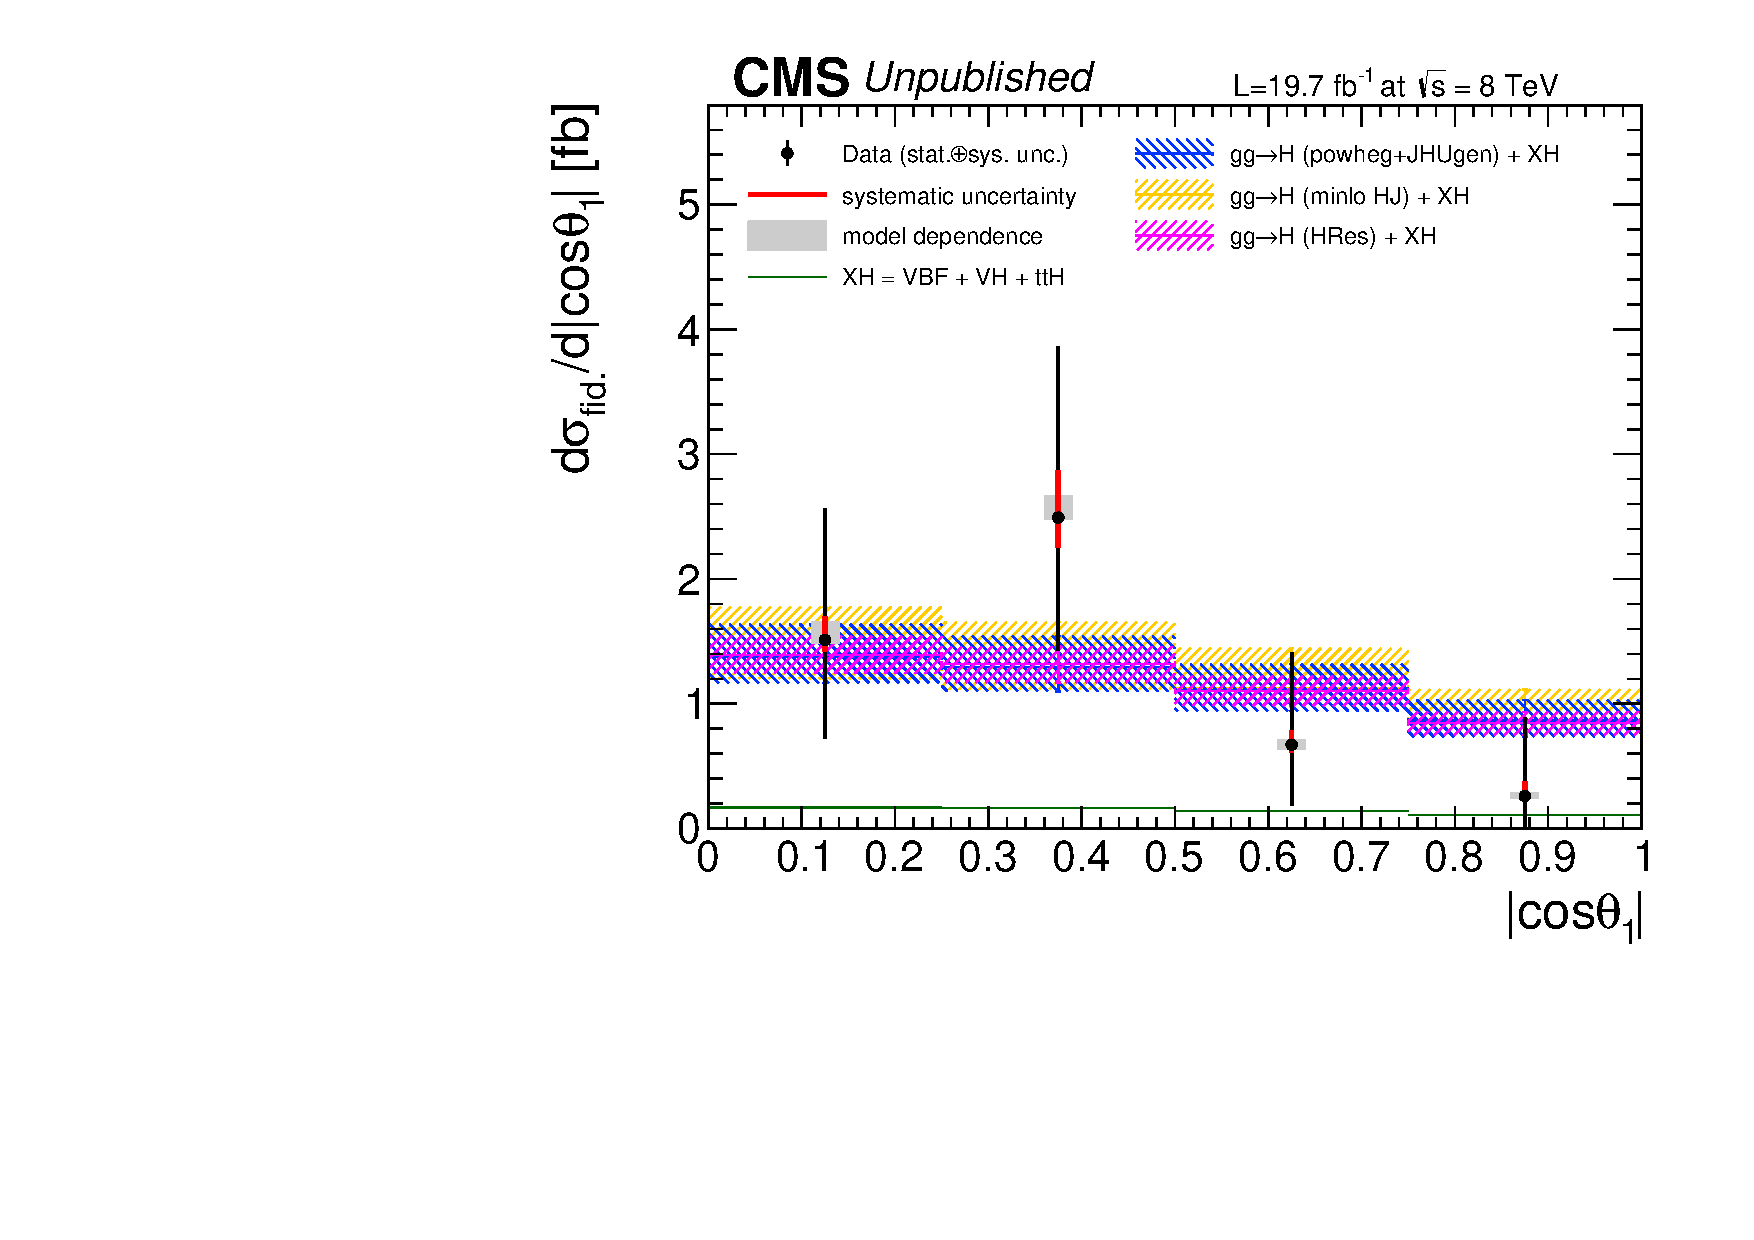
\includegraphics[width=0.30\textwidth,angle=0]{Plots/cosTheta1_unfoldwith_SM_125_unpublished.pdf}
      \label{fig:differential-results-2:b}
    }
    \subfigure[$|\cos \theta_{2}|$]{
      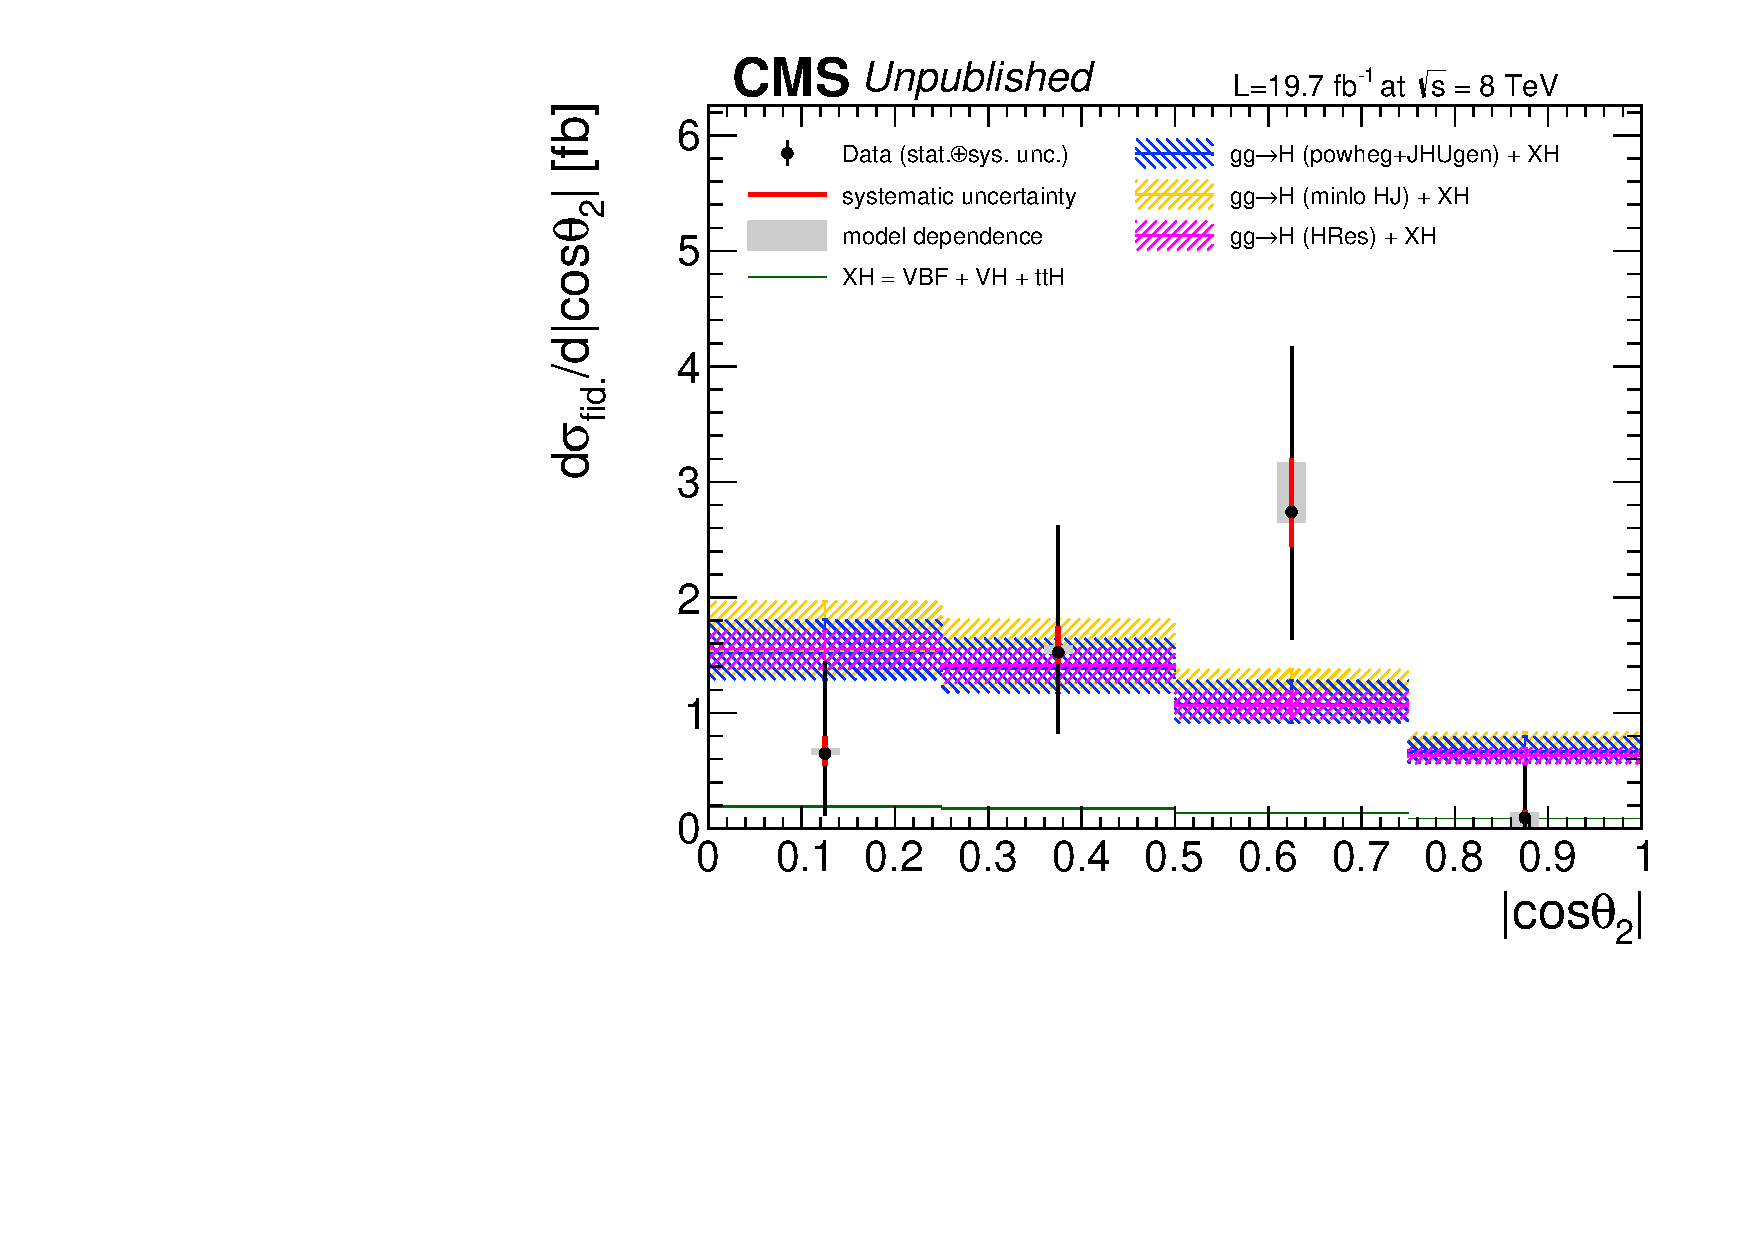
\includegraphics[width=0.30\textwidth,angle=0]{Plots/cosTheta2_unfoldwith_SM_125_unpublished.pdf}
      \label{fig:differential-results-2:c}
    } \\
    \subfigure[$|\Phi|$]{
      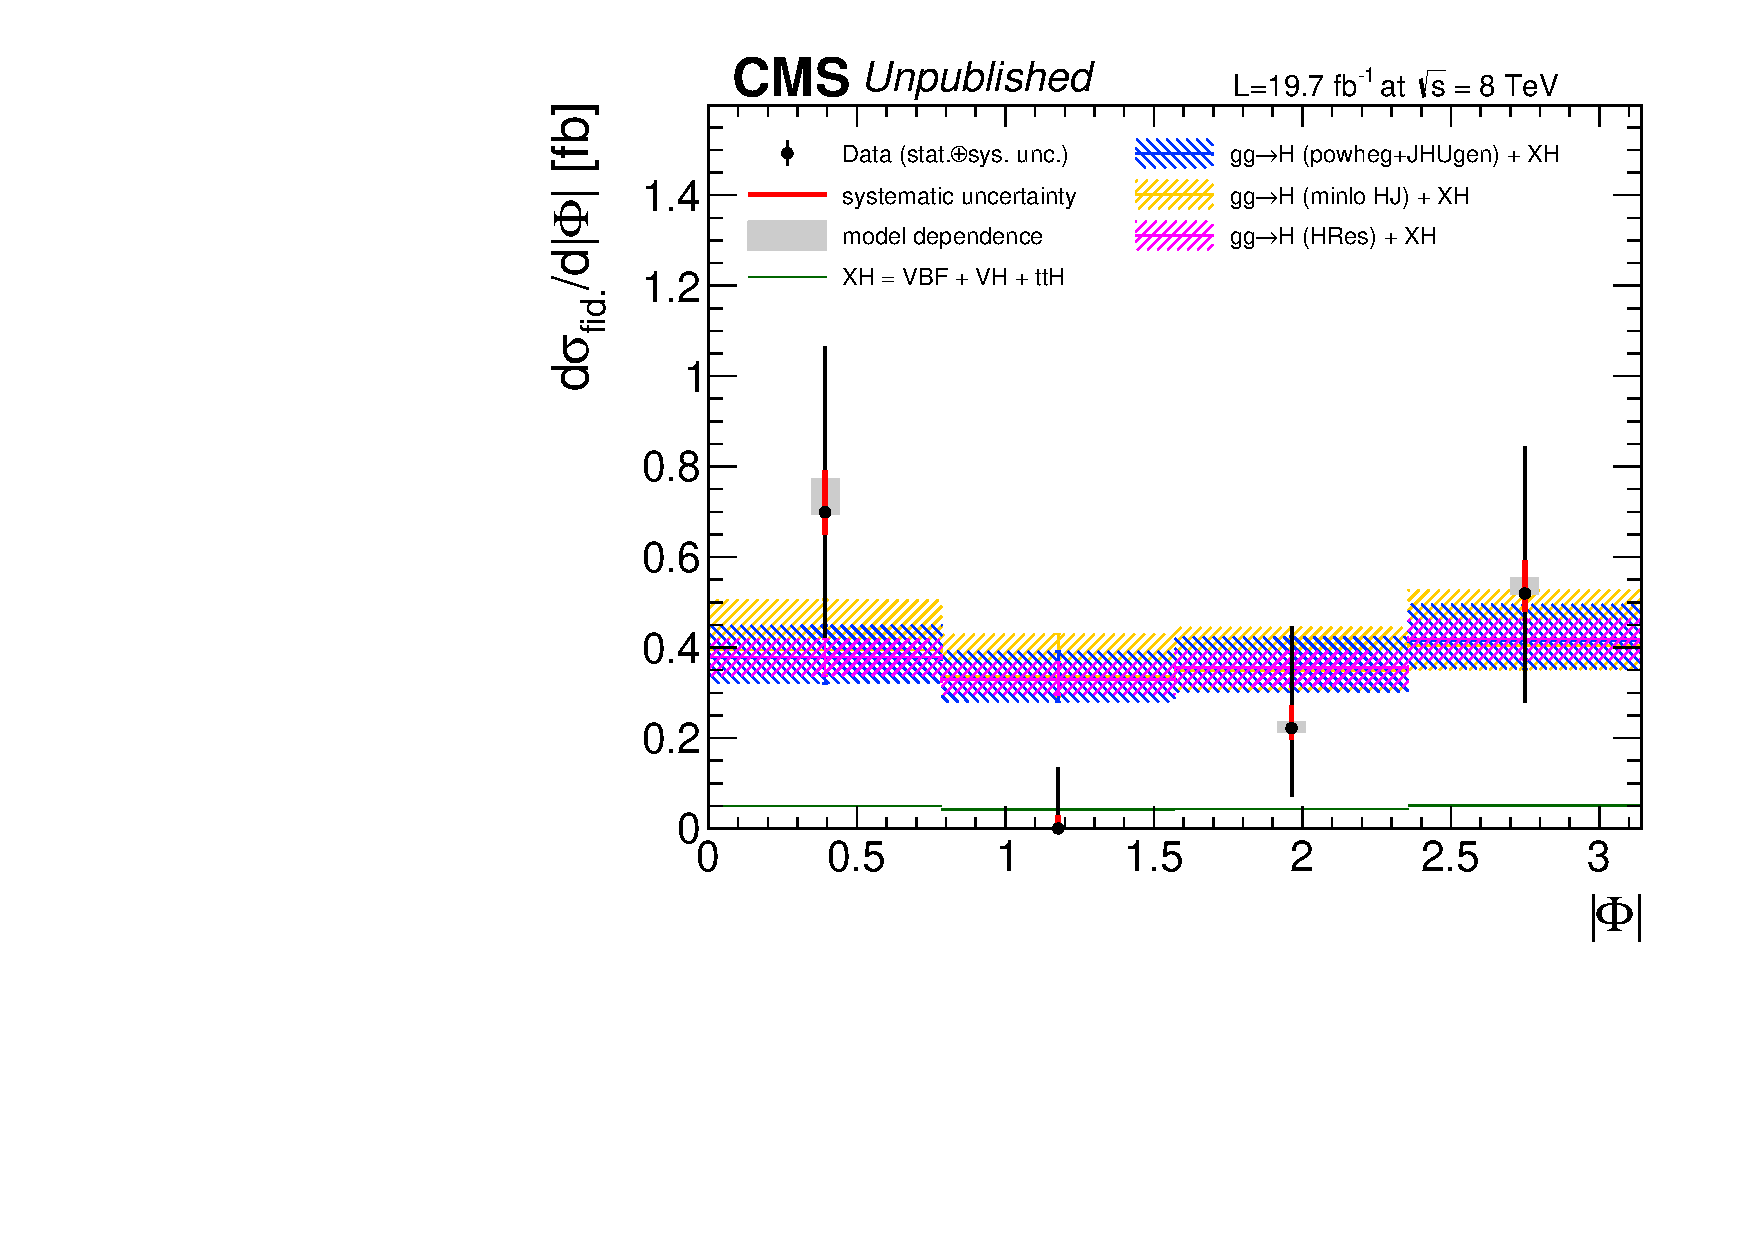
\includegraphics[width=0.30\textwidth,angle=0]{Plots/Phi_unfoldwith_SM_125_unpublished.pdf}
      \label{fig:differential-results-2:d}
    }
    \subfigure[$|\Phi_{1}|$]{
      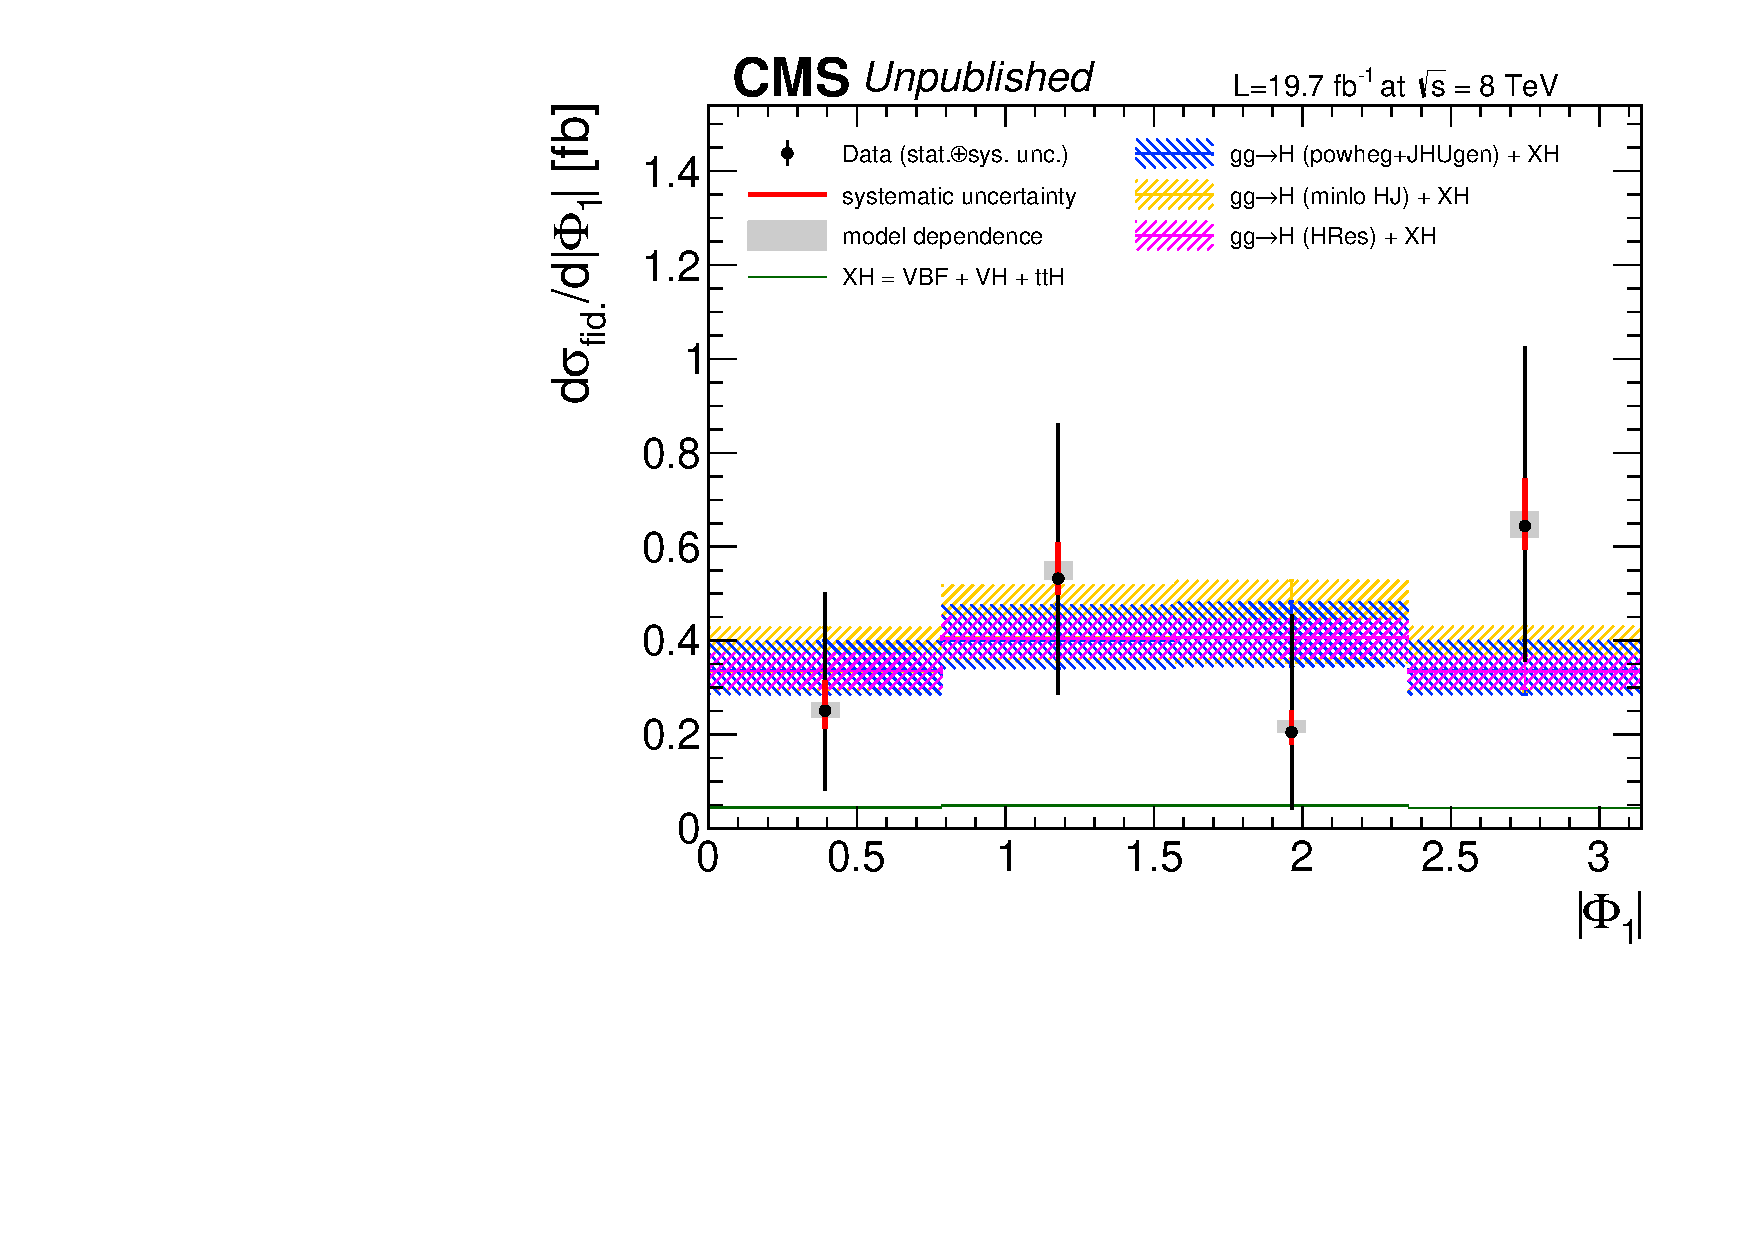
\includegraphics[width=0.30\textwidth,angle=0]{Plots/Phi1_unfoldwith_SM_125_unpublished.pdf}
      \label{fig:differential-results-2:e}
    } \\
    \subfigure[$\mathrm{m}(\mathrm{Z}_{1})$]{
      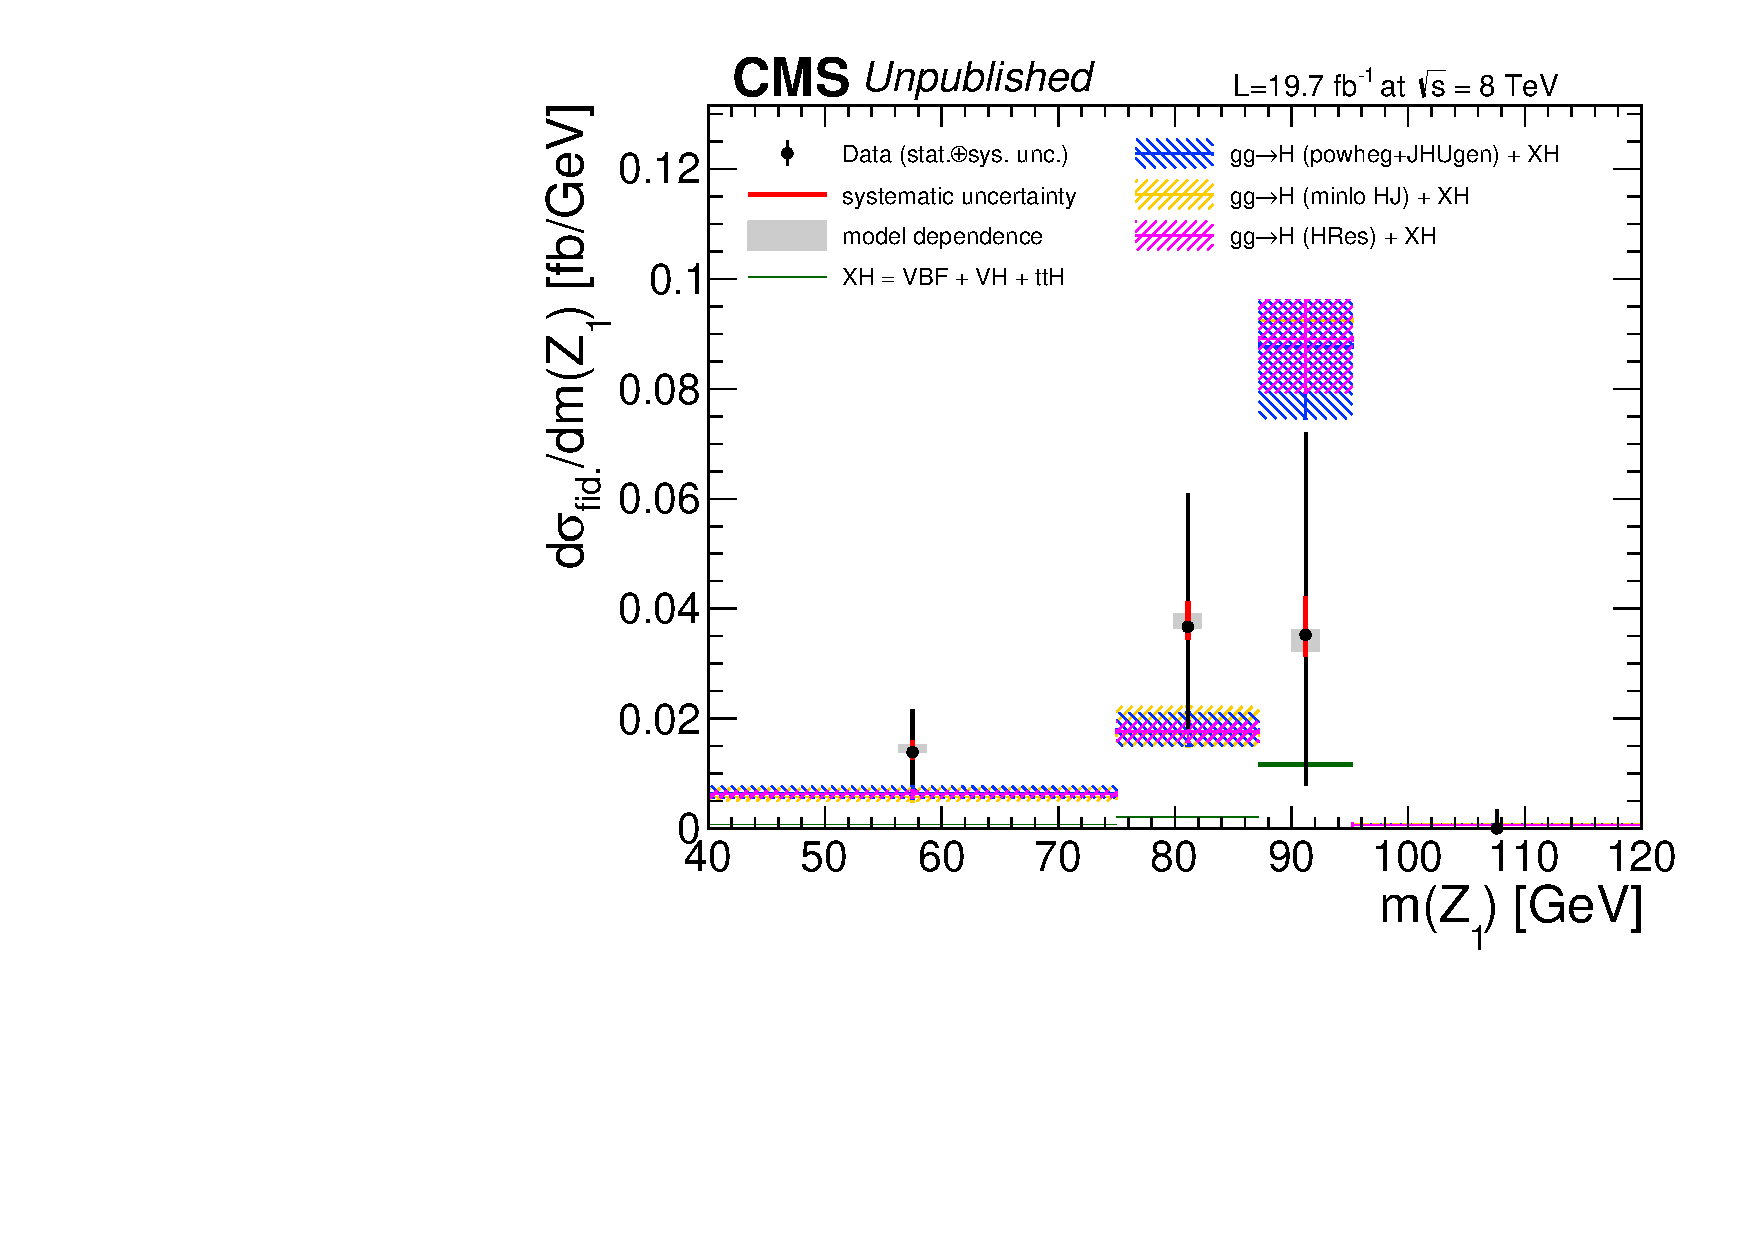
\includegraphics[width=0.30\textwidth,angle=0]{Plots/massZ1_unfoldwith_SM_125_unpublished.pdf}
      \label{fig:differential-results:f}
    }
    \subfigure[$\mathrm{m}(\mathrm{Z}_{2})$]{
      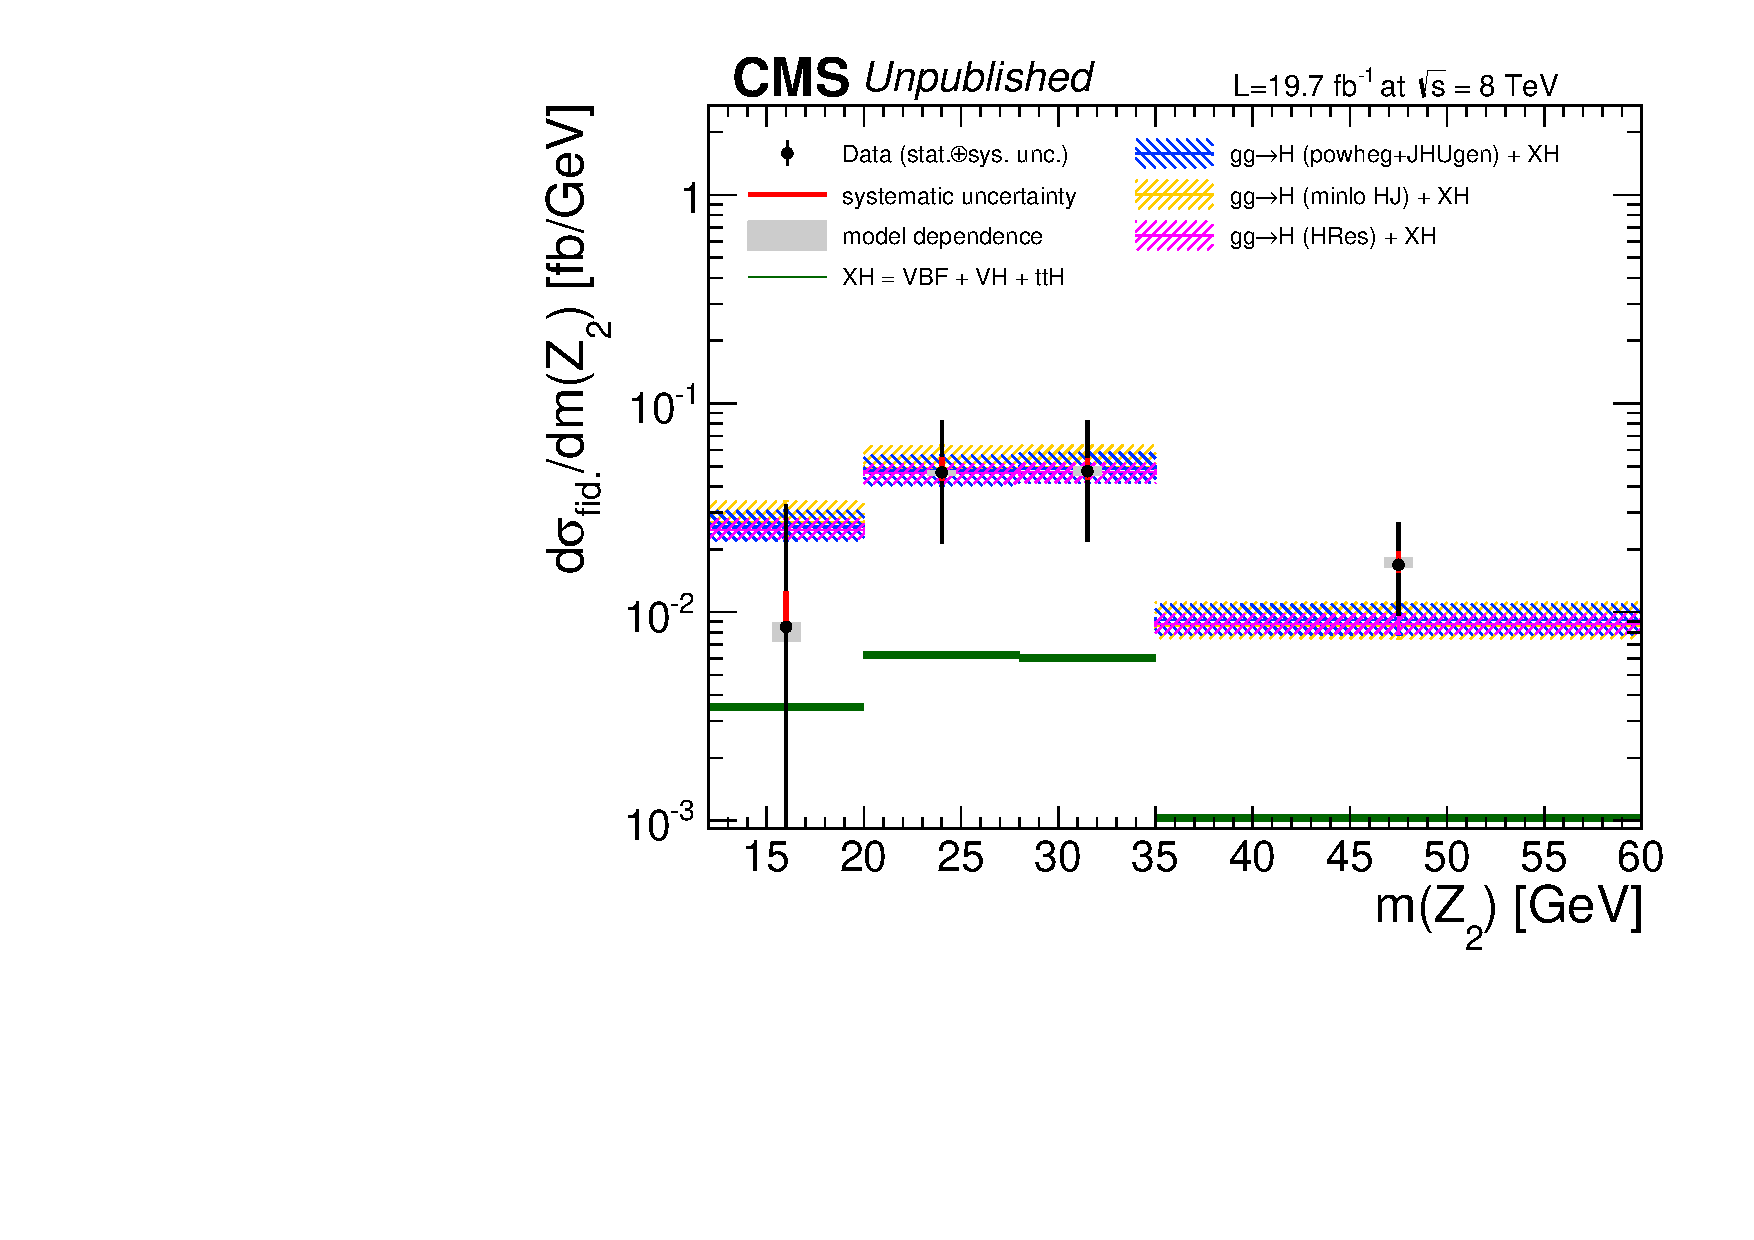
\includegraphics[width=0.30\textwidth,angle=0]{Plots/massZ2_unfoldwith_SM_125_logscale_unpublished.pdf}
      \label{fig:differential-results:g}
    }     
        \caption{The differential fiducial cross section results of $\Hllll$ and comparison with the theoretical predictions. 
        Systematic uncertainty is indicated by red bars while black bars shows the total statistical and systematic uncertainties, combined in quadrature.
        The model dependence is shown as an additional systematic uncertainty by the grey boxes.  The pink, yellow and blue colors shows
        the theoretical predictions, where acceptance of the 
        dominant $\ggH$ production mode is calculated by {\sc HRes},{\sc powheg minlo-HJ}+{\sc Pythia} and  {\sc powheg+JHUgen}+{\sc Pythia} respectively.
        The sub-dominant production contributions XH $=$ VBF $+$ VH $+$ $\ttH$ are shown in green separately. The total inclusive cross section is 
        normalized to the SM estimate computed at NNLL+NNLO accuracy for all theoretical predictions. The systematic uncertainties correspond to the 
        generators accuracy are also taken in to account for differential predictions. The fraction of $4e,4\mu$ and $2e2\mu$ in each bin is allowed 
        to float in the fit.
    }
  \label{fig:differential-results-2}
 \end{center}
\end{figure}
